\documentclass[12pt,a4paper,twoside,openright]{report}


\usepackage[pdfborder={0 0 0}]{hyperref}    % turns references into hyperlinks
\usepackage[margin=25mm]{geometry}  % adjusts page layout
\usepackage{graphicx}  % allows inclusion of PDF, PNG and JPG images
\usepackage{verbatim}
\usepackage{docmute}   % only needed to allow inclusion of proposal.tex
\usepackage{url}
\usepackage[parfill]{parskip}
\usepackage{booktabs}
\usepackage{fixltx2e}
\usepackage{amsmath}
\usepackage{amsthm}
\usepackage{listings}
\usepackage{array}
\usepackage[font={it},justification={centering}]{caption}
\usepackage{float}
\usepackage{framed}


\usepackage{fancyvrb,newverbs,xcolor}


\usepackage[UKenglish]{babel}% Recommended
\usepackage[bibstyle=numeric,citestyle=numeric,backend=biber,natbib=true]{biblatex}

\addbibresource{refs.bib}% Syntax for version >= 1.2


\raggedbottom                           % try to avoid widows and orphans
\sloppy
\clubpenalty1000%
\widowpenalty1000%

\renewcommand{\baselinestretch}{1.1}    % adjust line spacing to make
                                        % more readable


  
\lstdefinelanguage{Typescript}{
	keywords={break, case, catch, continue, debugger, default, delete, do, else, finally, for, function, if, in, instanceof, new, return, switch, this, throw, try, typeof, var, void, while, with},
	keywordstyle=\color{blue}\bfseries,
	ndkeywords={interface, class, extends, export, void, number, boolean, throw, implements, import, this},
	ndkeywordstyle=\color{orange}\bfseries,
	identifierstyle=\color{black},
	sensitive=false,
	comment=[l]{//},
	morecomment=[s]{/*}{*/},
	commentstyle=\color{purple}\ttfamily,
	stringstyle=\color{red}\ttfamily,
	morestring=[b]',
	morestring=[b]"
}

\lstset{
	language=Typescript,
	backgroundcolor=\color{cverbbg},
	extendedchars=true,
	basicstyle=\footnotesize\ttfamily,
	showstringspaces=false,
	showspaces=false,
	numbers=left,
	numberstyle=\footnotesize,
	numbersep=9pt,
	tabsize=2,
	breaklines=true,
	showtabs=false,
	captionpos=b
}


\definecolor{cverbbg}{gray}{0.85}
\newenvironment{cverbatim}
 {\SaveVerbatim{cverb}}
 {\endSaveVerbatim
  \flushleft\fboxrule=0pt\fboxsep=.5em
  \colorbox{cverbbg}{\BUseVerbatim{cverb}}%
  \endflushleft
}
\newenvironment{lcverbatim}
 {\SaveVerbatim{cverb}}
 {\endSaveVerbatim
  \flushleft\fboxrule=0pt\fboxsep=.5em
  \colorbox{cverbbg}{%
    \makebox[\dimexpr\linewidth-2\fboxsep][l]{\BUseVerbatim{cverb}}%
  }
  \endflushleft
}
\newcommand{\ctexttt}[1]{\colorbox{cverbbg}{\texttt{#1}}}
\newverbcommand{\cverb}
  {\setbox\verbbox\hbox\bgroup}
  {\egroup\colorbox{cverbbg}{\box\verbbox}}
  
  
  
\begin{document}




%%%%%%%%%%%%%%%%%%%%%%%%%%%%%%%%%%%%%%%%%%%%%%%%%%%%%%%%%%%%%%%%%%%%%%%%
% Title


\pagestyle{empty}

\rightline{\LARGE \textbf{Joshua Send}}

\vspace*{60mm}
\begin{center}
\Huge
\textbf{Conflict Free Document Editing with Different Technologies} \\[5mm]
Computer Science Tripos -- Part II \\[5mm]
Trinity Hall \\[5mm]
\today  % today's date
\end{center}

%%%%%%%%%%%%%%%%%%%%%%%%%%%%%%%%%%%%%%%%%%%%%%%%%%%%%%%%%%%%%%%%%%%%%%%%%%%%%%
% Proforma, table of contents and list of figures

\pagestyle{plain}

\chapter*{Proforma}

{\large
\begin{tabular}{ll}
Name:               & \bf Joshua Send                       \\
College:            & \bf Trinity Hall                     \\
Project Title:      & \bf Conflict Free Document Editing with Different Technologies \\
Examination:        & \bf Computer Science Tripos -- Part II, June 2017  \\
Word Count:         & \bf 1587\footnotemark[1]			\\
Project Originator: & Joshua Send                    \\
Supervisor:         & Stephan Kollmann                    \\ 
\end{tabular}
}
\footnotetext[1]{This word count was computed
by \texttt{detex diss.tex | tr -cd '0-9A-Za-z $\tt\backslash$n' | wc -w}
}
\stepcounter{footnote}


\section*{Original Aims of the Project}


TODO\footnote{A normal footnote without the
complication of being in a table.} 


\section*{Work Completed}

TODO

\section*{Special Difficulties}

TODO
 
\newpage
\section*{Declaration}

I, Joshua Send of Trinity Hall, being a candidate for Part II of the Computer
Science Tripos [or the Diploma in Computer Science], hereby declare
that this dissertation and the work described in it are my own work,
unaided except as may be specified below, and that the dissertation
does not contain material that has already been used to any substantial
extent for a comparable purpose.

\bigskip
\leftline{Signed TODO [signature]}

\medskip
\leftline{Date TODO [date]}

\tableofcontents

\listoffigures

\newpage
\section*{Acknowledgements}

TODO

%%%%%%%%%%%%%%%%%%%%%%%%%%%%%%%%%%%%%%%%%%%%%%%%%%%%%%%%%%%%%%%%%%%%%%%
% now for the chapters

\pagestyle{headings}

\chapter{Introduction}

Real time interaction between users is becoming an increasingly important feature to many applications, from word processing to CAD to social networking. This dissertation examines trade offs that should be considered when applying the prevailing technologies that enable concurrent use of data in applications. More specifically, this project implements and analyzes a concurrent text editor based on Convergent Replicated Data Types (also known as Conflict-free Replicated Data Types), CRDT in short, in comparison to an existing editor exploiting Operational Transformations (OT) as its core technology.


\section{Motivation}

Realtime collaborative editing was first motivated by a demonstration in the Mother of All Demos by Douglas Engelbart in 1968 \cite{MotherDemo}. From that time, it took several decades for implementations of such editing systems to appear. Early products were released in the 1990's, and the 1989 paper by Gibbs and Ellis \cite{Ellis1989} marked the beginning of extended research into operational transformations. Due to almost 20 years of research, OT is a relatively developed field and has been applied to products that are commonly used. The most familiar of these is likely to be Google Docs\footnote{https://docs.google.com}, which seems to behave in a predictable and well understood way. One reason Google Docs is so widely used might be that it follows users' expectations for how a concurrent, multi-user document editor should work. Importantly, this includes lock-free editing and independence of a fast connection, no loss of data, and the guarantee that everyone ends up with the same document when changes are complete. These are in fact the goals around which OT and CRDTs have developed.

The convergence, or consistency, property above is the hardest to provide -- it is easy to create a system where the last writer wins, but data is lost in the process. In a distributed system such as a shared text editor, the CAP theorem tells us we cannot guarantee all three of consistency, availability, and partition-tolerance \cite{Gilbert2005}. However, if we forgo strong consistency guarantees and settle for eventual consistency, we are able provide all three \cite{zeller2014}. As we will see, achieving eventual consistency is non-trivial. The two prevailing approaches that enable it, operational transformations and commutative replicated data structures, are discussed in detail the Preparation section.


\section{Overview}
This project aims to examine the trade-offs made when implementing highly distributed and concurrent document editing with Operational Transformations (OT) versus with Convergent Replicated Data Types (CRDTs). To do this I have designed experiments which expose statistics about network and processor usage, memory consumption, and scalability, and run these experiments on an environment built around the open source library ShareJS (which implements OT) along with a comparative system I created based on a specific CRDT. The system meets the originally proposed goals of implementing a concurrent text editor based on CRDTs which passes various tests for correctness; quantitative analysis is presented in the Evaluation section [section ref].

The custom CRDT on which the collaborative text editor is based is described in detail in the Implementation [section ref] section. In contrast to the OT-based library ShareJS, my system also runs on a peer to peer network architecture instead of a traditional client-server model. The lack of a server reduces the number of stateful parts in the system, at the expense of more complex networking. I managed this complexity by using a simulated peer to peer architecture. The simulation allows me to control the precise topology, link latencies, and protocol and explore advantages and disadvantages of using a P2P approach. 

One extension, adding undo functionality to the CRDT, was also completed. I developed two approaches which implement different semantics and consistency models and were developed originally, before reading related literature. However, one paper, Logoot-Undo, takes a very similar approach and is discussed briefly below.

\section{Related Work}

Part of the challenge of this project was to develop my CRDT and associated algorithms based only on an explanation of the required functionality provided by Martin Kleppmann. As a result, my solution is not optimal in all aspects, and could be improved upon in the future. Several possible optimizations are discussed in the Implementation section [TODO, section ref]. It also falls into the class of `tombstone' CRDTs, marking elements as deleted rather than fully removing them, which forces the data structures to grow continuously over time [perhaps put a mention of treedoc's commit protocol and and a reference to using vector clocks to remove tombstones]). Other CRDTs are `tombstone-free' and do not suffer from this unbounded growth. Existing CRDTs of both types are discussed here.

\subsection{Treedoc}

Treedoc \cite{preguica2009} is a replicated text buffer; an ordered set that supports insert-at and delete operations. This CRDT gets its name from the tree structure used to encode identifiers and order elements in the set. Each node in the tree contains at least one character, and the string contained in the buffer is retried using infix traversal. Each client has a copy of the same tree, and can insert new nodes at any time. Two concurrent inserts at the same node are merged as two `mini-nodes' within one tree node. Each insert is tagged with a unique client identifier which comes from an ordered space. Using the identifier order in combination with infix traversal creates a total ordering over the characters contained in the tree. With the total order, all clients with copies of the tree will retrieve the same string from their Treedoc. Having a total order is an important property used to guarantee eventual consistency in CRDTs. Using unique, ordered client IDs to provide a total order in concurrent cases is common in CRDT design and indeed used in my own CRDT.

\begin{figure}[htb]
\centering
  \begin{tabular}{ >{\centering}m{6cm} >{\centering}m{15mm} >{\centering\arraybackslash}m{6cm} }
    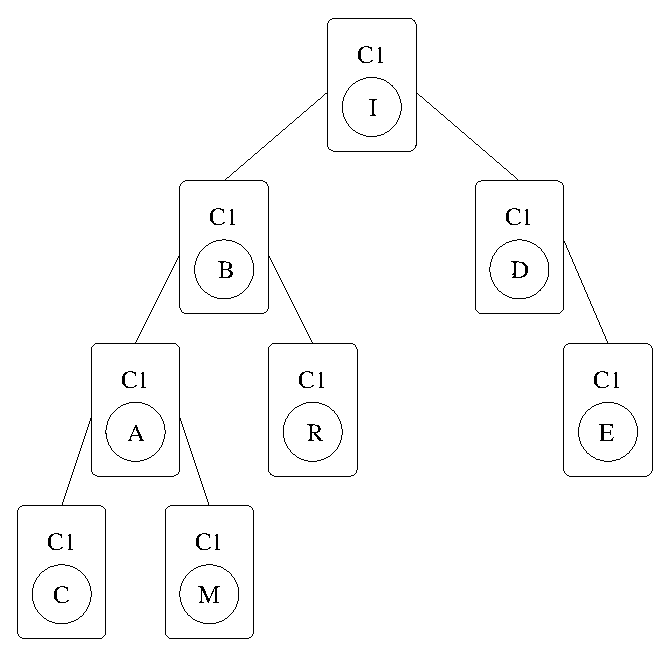
\includegraphics[width=1\linewidth]{figs/treedoc_1.eps}  &
    $\longrightarrow$  &
    \includegraphics[width=1\linewidth]{figs/treedoc_2.eps}
  \end{tabular}
\caption{Concurrent updates to the same node. In the first state (left), client 1 has written the string `Cambride' into the text buffer. The systems settles and client 2 also sees the string `Cambride'. Both clients 1 and 2 realize there is a missing character -- client 1 inserts `g' and client 2 mistakenly inserts 'h'. As both create the same node in the tree, the nodes are merged as mini-nodes into a larger node. Both clients now see the string 'Cambridghe'.}
\label{fig:treedoc}
\end{figure}

Deletes in Treedoc are handled by marking a node as deleted (but the node remains in the structure). Thus Treedoc falls into the class of `tombstone' CRDTs. As deletes and inserts are not guaranteed to result in a balanced tree, the authors propose an expensive commitment protocol to rebalance it. Not only is this inefficient, but also rather contrary to the spirit of CRDTs.

\subsection{Logoot}

Logoot \cite{weiss2008} belongs to the class of text CRDTs which do not require tombstones for deletion. It achieves this by totally ordering identifiers, rather than relying on implicit causal dependencies between identifiers (which Treedoc embeds in the tree's branches). Logoot does generate identifiers using a tree, but each identifier contains the full path in the tree, which frees it of dependence on other nodes. This means that to delete, any client can simply remove the identifier and the data it tags.

Logoot also favors marking larger blocks of text with identifiers, rather than per-character. This, in combination with not needing tombstones, promises major efficiency gains over CRDTs such as Treedoc. Even further, two papers \cite{nedelec2013lseq} \cite{nedelec2013} offer optimizations beyond the basic Logoot implementation by improving the strategy used to allocate new identifiers in the generator tree. However, these algorithms are specific to Logoot and of little relevance to this project.

Logoot is important as an example of a tombstone-free CRDT for text. Additionally, subsequent research enabled `undo' and `redo' functionality for this CRDT, which is described below.


\subsection{Logoot-Undo}

CRDTs generally struggle to provide an undo mechanism since the concept of reversing an update to the data structure is fundamentally contrary to the key property of CRDTs: commutativity of operations. For example, reversing an insert is not commutative with the original insertion. If it were, the removal of a nonexistent element, followed by its insertion would have to result in the same thing as insertion followed by removal. In the first case, the element is present, while in the second it is removed. These outcomes clearly are not the same.

Logoot Undo \cite{weiss2010undo} proposes to resolve this by essentially tagging each identifier with a $visible$ counter. An undo of an insertion would decrement it, while redo would increment it. If the $visible$ counter is positive, the characters are visible. As discussed in [REFERENCE NEEDED], this leads to some rather unexpected behavior. However, this approach is viable since increments and decrements commute and guarantee eventual convergence. In Logoot Undo, any client can undo any other client's operations which is called global undo. The use of a counter is identical to the undo mechanism I developed independently, though I chose to implement a local undo rather than global one, where clients can only undo their own operations.


\chapter{Preparation}


\section{Consistency Models}

	\subsection{What is ``Conflict Free''}
	
	One important definition is the exact meaning of ``conflict free''. There appears to be more than one way of interpreting it. On one hand, there is the user's intuitive idea that any of their own operations should behave as if they were the only users on the system. On the other hand, there is the data-centric view of conflict. In this case, operations conflict if they are concurrent and modify the same data or index in a text buffer. Conflict free then means that no data is lost, and after all operations are exchanged the resulting states agree.
	
	The common conflicting operations in text editing are inserting characters into the same index of a shared text buffer, or simultaneously deleting the same characters. The second is easy to make conflict-free, and both the user and data oriented definitions of conflict agree -- deleting a character concurrently or on a single user system should still result in the character disappearing. In the case of inserting text into the same index, the definitions cannot agree. Both users expect their own text to appear in the index they inserted at. However, in order to satisfy the data-centric definition we are not allowed to lose data, and must eventually present both users with the same string. The solution is to let one user `win' and insert their characters at the desired index, and shift the other users' characters to appear after. Both operational transformations and CRDTs achieve this in fundamentally different ways. This entire process is demonstrated in  \ref{fig:reconcile}.
	
	\begin{figure}[htb]
	\centering
	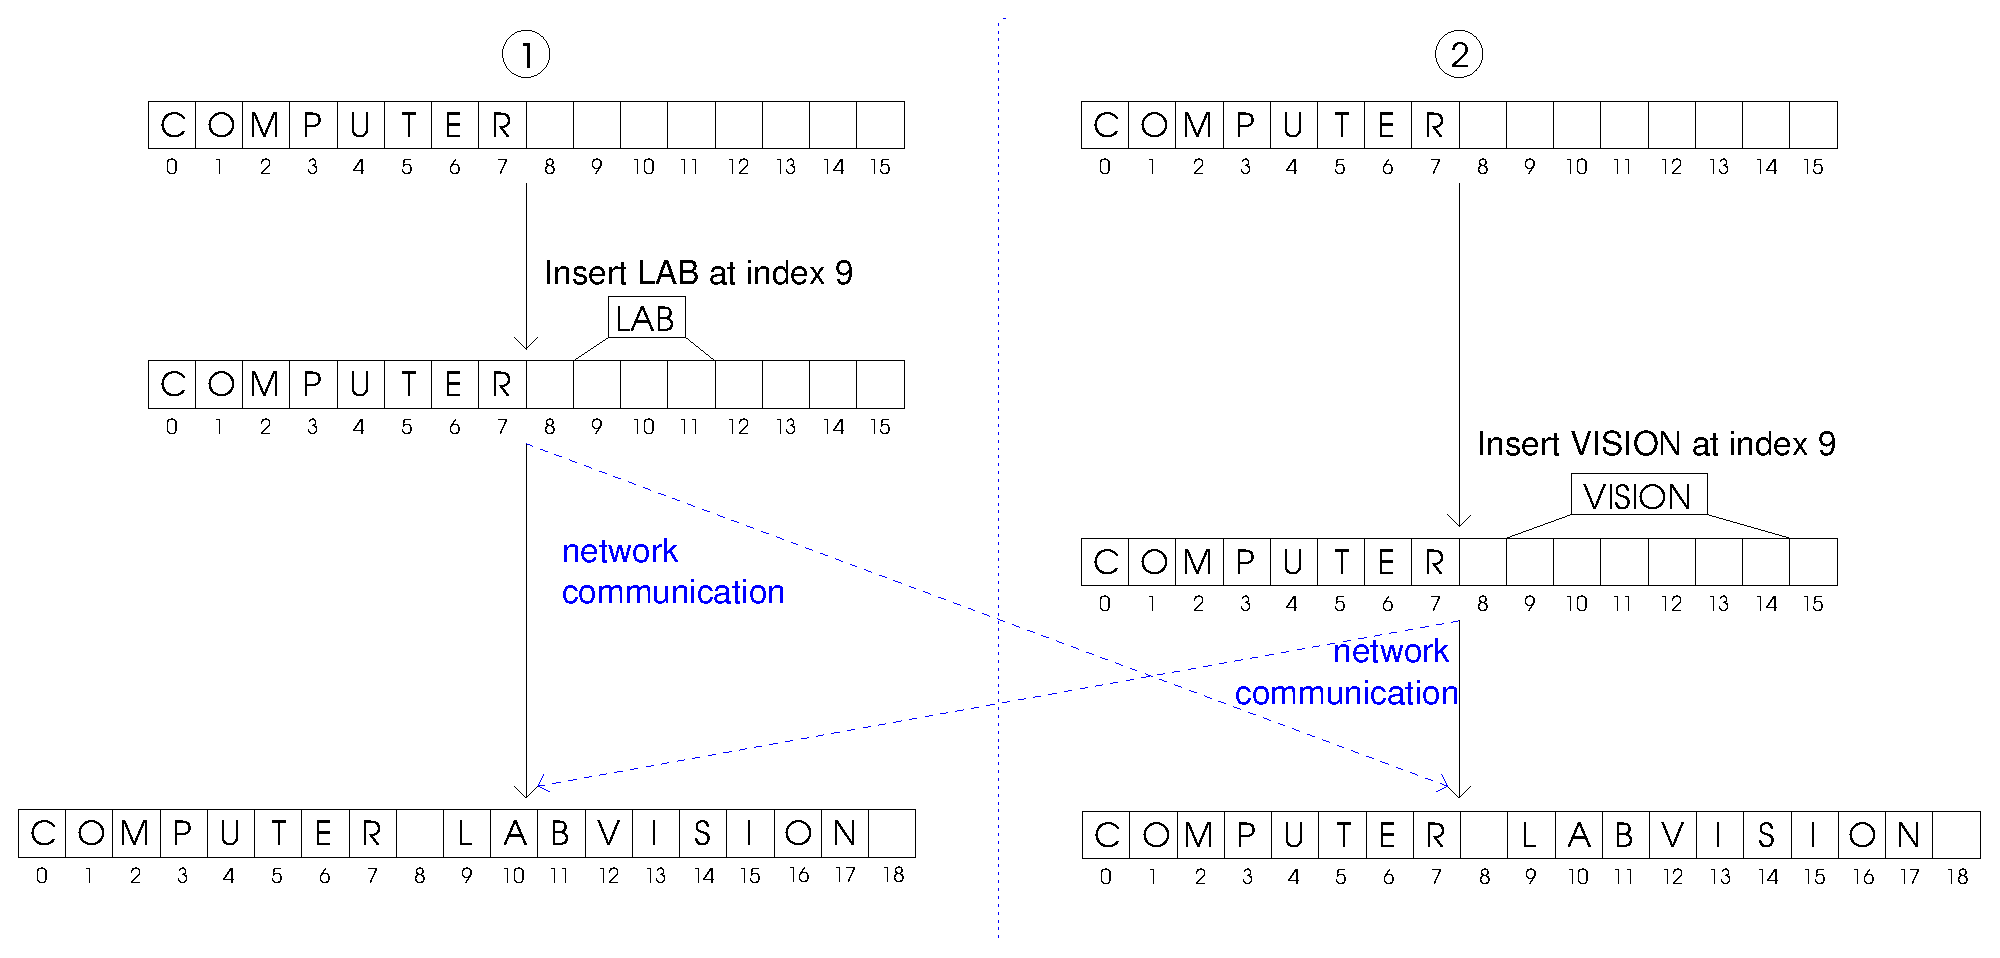
\includegraphics[width=1\linewidth]{figs/reconcile.eps}
	\caption{Two clients are initially in a quiescent state i.e. the system has settled with the shared string `computer '. They then concurrently insert different words at the same index. At first each sees only their own edit. Then operations are exchanged and the system reaches quiescence again. Both clients see the string 'computer labvision'. Client 1 thus `won' and kept the original index, while Client 2 had its insertion offset.}
	\label{fig:reconcile}
	\end{figure}
	
	\subsection{CCI Consistency Model}
	The commonly used consistency model for concurrent document editing is the CCI model. The definition here is borrowed from \cite{weiss2010undo}.
	
	\begin{itemize}
		\item \textbf{Consistency:} All operations ordered by a precedence relation, such as Lamport’s happened-before relation \cite{lamport1978}, are executed in the same order on every replica.
	
		\item \textbf{Convergence:} The system converges if all replicas are identical when the system is idle.
		
		\item \textbf{Intention Preservation:} The expected effect of an operation should be observed on all replicas. This is commonly accepted to mean:

			\begin{itemize}
				\item \textit{delete}  A deleted line must not appear in the document unless the deletion is undone.
				
				\item \textit{insert}  A line inserted on a peer must appear on every peer; the order relation between the document lines and a newly inserted line must be preserved on every peer.
				
				\item  \textit{undo}  Undoing a modification makes the system return to the state it would have reached if this modification was never produced.
				
			\end{itemize}	
		
	\end{itemize}
	
	The given definition of intention preservation is accepted, but may produce some unexpected results as we will see when discussing Undo in [reference needed].
	

\section{Achieving Eventual Consistency}

	As mentioned briefly in the prior section, operational transformations and CRDTs aim to achieve eventual convergence on all clients. The common conflicting operations that must be given special consideration are concurrently inserting characters at the same index, and deleting the same character, and deleting a character while removing characters before it.

	\subsection{Operational Transformations}
	
	The easiest way to understand operational transformations is by example.
	
	
	Figure \ref{fig:ot1} demonstrates the \textit{concurrent insert at same index} case.
	
	\begin{figure}[H]
	\centering
	\includegraphics[width=1\linewidth]{figs/ot1.eps}
	\caption[Operational Transformations -- concurrent insertion]{This figure shows how operational transformations might handle concurrent insertion at the same index. Here, both clients insert different strings after index 5. The operations are exchanged, and the key \textit{transform} function (in green) detects the conflict, and chooses to offset `` world'' on Client 1 by 6 (in red), which is the length of its own previously inserted string `` there ''. On Client 2, once the insert `` there '' arrives, the algorithm knows not to offset it (due to some arbitrary ordering such as client ID) and places it at index 5. Thus both clients resolve the string ``Hello there world''}
	\label{fig:ot1}
	\end{figure}
	
	Figure \ref{fig:ot2} demonstrates the \textit{concurrent deletion of same character} case.

	\begin{figure}[H]
	\centering
	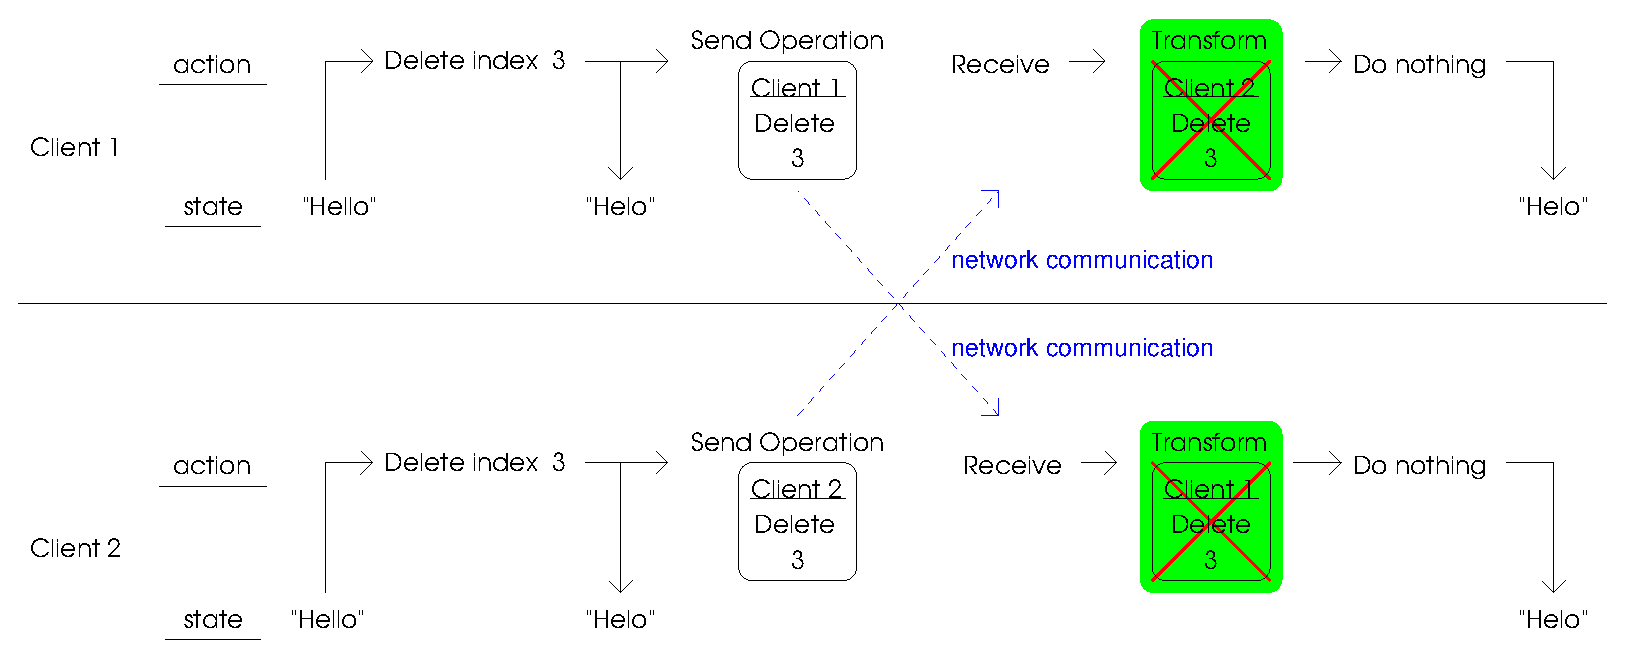
\includegraphics[width=1\linewidth]{figs/ot2.eps}
	\caption[Operational Transformations -- concurrent deletion]{Both clients concurrently delete index 3 of ``Hello'', resulting in ``Helo''. The operations are exchanged. The \textit{transform} function (in green) detects the conflict, and on both clients discards the remote operation. Integrating it would cause modifications the user did not execute (i.e. delete `o' in addition). By discarding the operations, both clients resolve ``Helo'' correctly.}
	\label{fig:ot2}
	\end{figure}
	
	Figure \ref{fig:ot3} demonstrates the \textit{concurrent insertion and deletion} case.
	

	\begin{figure}[H]
	\centering
	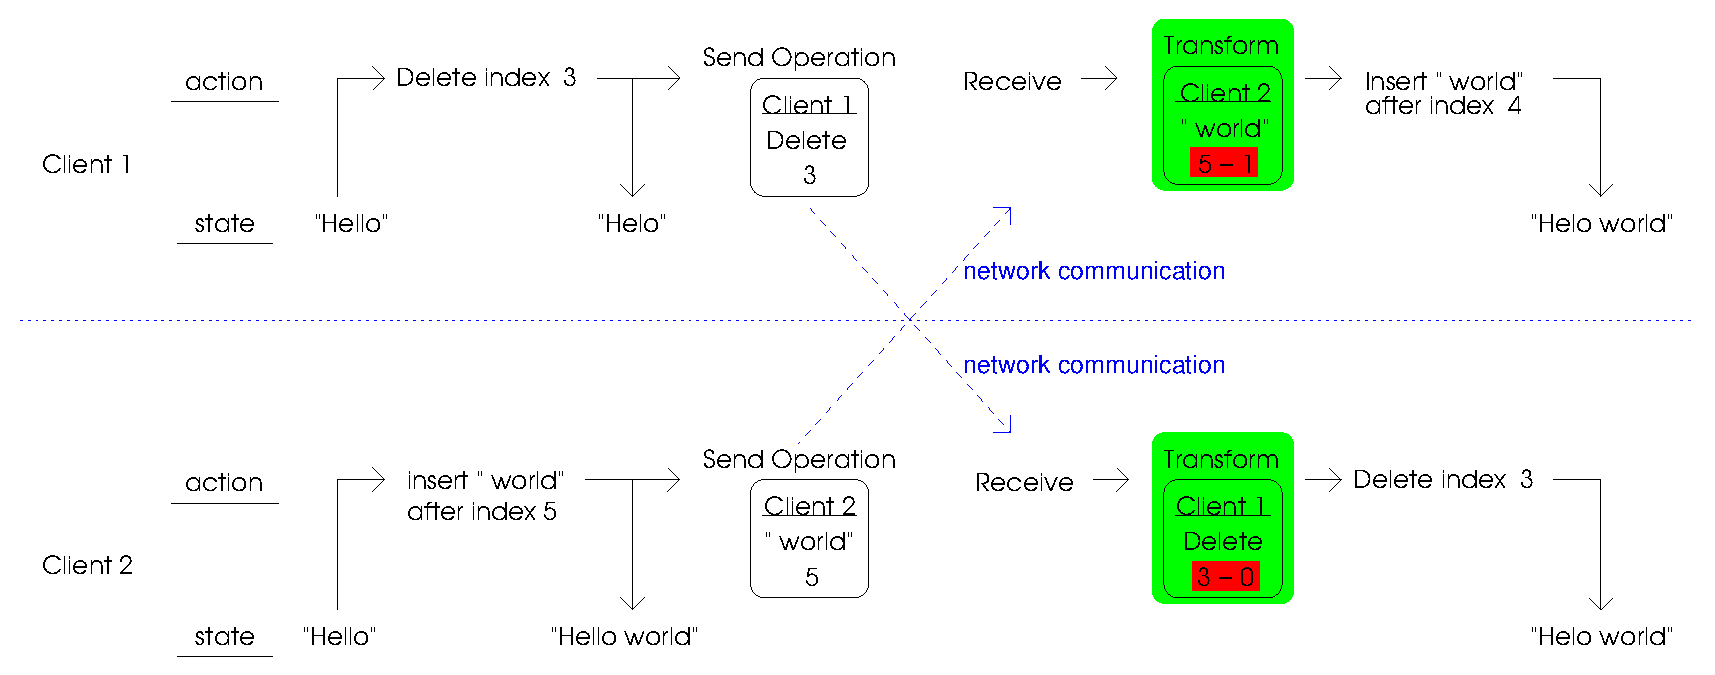
\includegraphics[width=1\linewidth]{figs/ot3.eps}
	\caption[Operational Transformations -- concurrent insertion and deletion]{Here Client 1 deletes index 3 of the initial string ``Hello'', resulting in ``Helo''. Meanwhile, Client 2 inserts `` world'' after index 5 resulting in ``Hello world''. The operations are exchanged. The \textit{transform} function (in green) detects the conflict, and on Client 1 knows to subtract 1 from the index to insert `` world'' after because a prior character has been deleted concurrently. On Client 2, there is no conflict and the delete can proceed at position 3. Thus both clients resolve ``Helo World'' correctly.}
	\label{fig:ot3}
	\end{figure}


	
	
		
	\subsection{Convergent Replicated Data Types}
	
	This section will provide an intuition for CRDTs for text editing in general, while the specific CRDT used for this project is outlined in chapter 3 [reference needed].

	CRDTs, which were first formalized in a 2007 paper \cite{shapiro2007}, trade the complex algorithms used in OT for a more complex data structure. Rather than relying on a serial order provided by a server, or logic to transform operations against each other, operations are tagged with totally ordered identifiers which allow us to extract the data in the native form -- for example, a string will be represented as a set of tagged characters, so they may be read out according to the tag ordering. Figure~\ref{fig:taggedset} is a simple demonstration of how this works. 
	
	\begin{figure}[H]
	\centering
	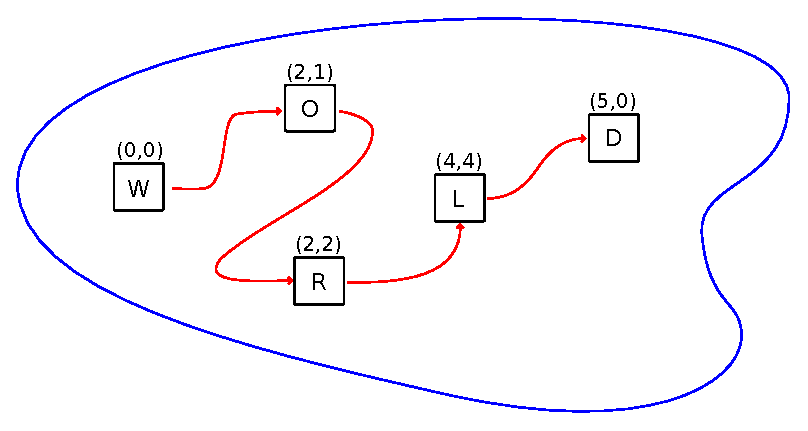
\includegraphics[width=1\linewidth]{figs/tagged_set.eps}
	\caption[Text CRDT as a tagged set]{A CRDT containing the word ``World''. The CRDT is a set of nodes that are tagged with ordered identifiers. The order used here is $<$, ordered by the first element of the pair, then by the second. The red arrows trace out the ordering, which presents the word ``World''.}
	\label{fig:taggedset}
	\end{figure}
	
	***NEED to incorporate partial order of operations??***
	
	There are technically two classes of CRDTs: state- and operation-based. State-based CRDTs disseminate the entire local state to other clients which is then merged into their copies. This requires that the merge operation be commutative, associative, and idempotent~\cite{shapiro2011}. Operation-based CRDTs relay modifications to other clients, which execute them on the local replica. These only require that all operations commute, and that the communication layer guarantees only-once, in order delivery~\cite{takada2013}. This project uses an operation-based CRDT, so the key property to fulfill is commutativity of operations while providing network layer delivery guarantees.
	
	If these requirements are met, all clients will to converge to an identical, ordered result. This follows from the fact that elements in the CRDT have a total order defined over them: as long as all modifications arrive intact, all clients can retrieve the correct data.

	\subsection{ShareJS}
	
	ShareJS~\cite{sharejs} is an open source Javascript library implementing Operational Transformations which can be deployed on web browsers or NodeJS\footnote{\url{https://nodejs.org/en/}} clients. It is the core resource around which I built the comparative system to collect statistics from. To this end, it is useful to know more precisely how ShareJS operates and what kind of behavior might be expected. As are a large variety of algorithms that can enable OT~\cite{kumawat2016}, rather than tracking down the papers ShareJS is based on, much of what is summarized below was deduced by reading its source code. Its core features are versioned documents, an active server which orders and transforms operations, and primary supported actions `insert' and `delete'.
	
	Replicated documents are versioned, and each operation applies to a specific version. The version number is used to transform operations against each other and detect concurrent changes. The supported operations are insert and delete, and the resulting modifications are sent as JSON to the server.
	
	An Insert operation for adding text at index 100 in document version 1:
\begin{lcverbatim}
{v:1, op:[{i:`Hello World', p:100}]}
\end{lcverbatim}

	A deletion of the world ``Hello'' at index 100:
\begin{lcverbatim}
{v:1, op:[{d:`Hello', p:100}]}
\end{lcverbatim}

	Multiple operations may be sent in one packet:
\begin{lcverbatim}
{v:1, op:[{d:`World', p:100}, {i:`Cambridge', p:110}]}
\end{lcverbatim}

\vspace{5mm}

	The library contains both client and a server code. The server provides a global, serialized order of operations to be applied on each client. The server also transforms concurrent operations against each other, but has the choice of rejecting an operation if the target document version is too old. In order to transform operations against each other, the server must maintain a list of past operations, which has an effect on memory consumption. This is confirmed in [reference needed to experiment].
	
	ShareJS clients can also only have one packet to be in flight to a server, which engenders the need for combining multiple operations in a single packet. However, this has implications for packet size and quantity as network latency grows [reference to experiment]. Additionally, since the server can reject operations that were generated and applied at a client, the clients must be able to undo rejected operations, as well as manage any subsequent, dependent operations that have occurred (this is one of the key parts of \textit{transformation} of operations). To enable this, the clients must each have a list of past operations, which also affects memory use [reference to experiment].

	
\section{Analysis}
	
	\subsection{Memory}
	
	***This can be redone, for instance ops grow in size as document number grows***
	
	Given our rough understanding of CRDTs and ShareJS, we can make hypotheses about the quantitative results that might be obtained. In terms of basic memory requirements, each ShareJS client requires storing the current document string, along with past operations. At worst, each character in the string was delivered as an individual operation, so given n characters we expect $O(2n)$ = $O(n)$ memory usage. The server must also store a list of these operations, but the overall cost is still $O(n)$. On the other hand, CRDTs at worst tag each character with a unique identifier. The largest identifier is $O(log(n))$ characters long (assuming increasing natural numbers as tags), which leads to $O(nlog(n))$ cost overall. This is slightly higher than ShareJS's linear growth.
	
	\subsection{Network}
	
	Given that the CRDT system will run over a P2P network, while ShareJS requires a server, as long as the P2P network is more connected than a star topology (equivalent to client/server), the average latency for all the clients to receive data should be lower. In fact, at best a P2P network will cut the time to receive an update to half of a client/server network. 
	
	In terms of number of characters sent over the network per action, it is difficult to make a prediction due to optimizations that may or may not be implemented. However, given a basic assumption of each character inserted into a CRDT also requiring an identifier to be sent, we get an $\Theta(nlog(n))$ space complexity again. On the other hand, ShareJS sends one character or word at a time, plus an index and a document version that the operation was performed on. If there are $n$ characters in the document, there are at most $n$ versions. The length of the decimal string $n$ is $log(n)$ characters. Thus we get an approximate $\Theta(nlog(n))$ packets sent for ShareJS.
	
	\subsection{Processor Load}
	
	The relative algorithmic simplicity of CRDTs versus OT hints that CRDTs should be computationally more efficient. If we assume that an insert and delete operation can be done in constant time in a CRDT, then the most expensive operation to be done is a linear time retrieval and update of the string displayed to the user. Operational transformations not only need to update the displayed string, but also need to transform (either on clients or on the server) changes against any concurrent edits. While this is hard to quantify, it is reasonable to expect that achieving convergence is more processor intensive with OTs than CRDTs.
	
	
	\subsection{Client-Server versus Peer to Peer}
	
	It is worth examining what other reasons there might be for using a system that is capable of running over a P2P network. Generally, a key element is privacy. A P2P network can run over a secure, anonymous network such as Tor\footnote{\url{https://www.torproject.org/docs/faq}} and since no middleware needs to intercept and read packets, encryption may be used. OT systems almost always require a server, which may need to transform operations against each other – which requires transmitting all operations in plain text and kills any hope of privacy. One benefit of using a central server is that there is a natural “cloud” repository in which to store the contents of documents; a P2P network either requires some peers to be connected in order to download the latest version, or a server to have a repository of documents. Similar issues face state replay for new clients that join an active network; this is examined in section [SECTION REF]. Luckily, in terms of privacy, a central repository for CRDT based documents would not need to be able to read the contents, just distribute them on demand. Lastly, established P2P networks have further benefits such as lacking single points of failure, lower probability of downtime and lower operational cost to the provider, but these properties and their implications are not in the scope of this project.
	
\section{Starting Point}

As stated in the proposal, I had prior experience with ShareJS, which was leveraged when creating the comparative system. Additionally, I was already proficient in Javascript and had working knowledge of Typescript, my main implementation language. However, almost all other aspects were new, notably: learning about CRDTs, writing test cases, the process of creating experiments and using these to profile performance, and how to implement a simulation.

As the project progressed, several courses contributed or reaffirmed ideas I could use. Notably, the Computer Systems Modeling \cite{compsysmodeling} course had a short section on simulation which aligned very well with what I had already implemented at the time. The Part IB course on Concurrent and Distributed Systems \cite{concdistsystems} provided valuable background towards Lamport and Vector clocks, causality, and total orderings in distributed systems; the IB Computer Networking course \cite{computernetworking} gave me a foundation and overview helpful for planning the network component of my system.


%Lastly, the Mobile and Sensor Systems course\footnote{\url{http://www.cl.cam.ac.uk/teaching/1617/MobSensSys/}} gave me some ideas when seeking alternatives to the flooding implemented in my network simulation.

\section{Requirements Analysis}
To reiterate the success criteria listed in the project proposal, I hoped to

\begin{enumerate}
\item Implement a concurrent, distributed text editor based on CRDTs 
\item Pass correctness tests for this CRDT
\item Obtain and compare quantitative results from ShareJS and the CRDT based systems
\end{enumerate}

Points one and three have multiple unspecified subgoals. For clarity, Table~\ref{table: goals} lists these and their respective importance and difficulty. The goals closely mirror the `Detailed Project Structure' of the proposal.

\begin{center}
\begin{table}[H]
\centering
\caption{Project Goals, Priority, and Difficulty}
\label{table: goals}
\begin{tabular}{@{}lll@{}}
Goal											 	& Priority & Difficulty \\ \toprule
Implement and unit test core CRDT                	& High     & Medium \\ \midrule
Implement network simulation                     	& High     & High   \\ \midrule
Optimize CRDT Insert                             	& Low      & Low    \\ \midrule
Design experiment format                         	& High     & Low    \\ \midrule
Create comparative ShareJS system					& High     & Medium \\ \midrule
Write log analysis scripts                       	& Medium   & Low    \\ \bottomrule
\end{tabular}
\end{table}
\end{center}



\section{Software Engineering}

	\subsection{Libraries}
	ShareJS \cite{sharejs} is the main external resource I required. It is released under the MIT license. I used the simpler ShareJS v0.6.3 rather than the more current ShareJS 0.7, also known as ShareDB. This package was installed via the NPM\footnote{\url{https://www.npmjs.com/}} package manager. The other large library I used was D3.js\footnote{\url{https://d3js.org/}}, a commonly used data visualization tool that helped me build a dynamic network graph for debugging purposes. I did a survey of other drawing libraries that might be simpler and lighter on resources, however in terms of documentation, ease of use, and familiarity I did not find anything more suitable.
	
	\subsection{Languages}
	The three main implementation languages, by lines of code, are Typescript\footnote{\url{http://www.typescriptlang.org/}}, Python 2.7\footnote{\url{https://www.python.org/}}, and Coffeescript/Javascript  (mainly in ShareJS). Reasons for choosing Typescript as the primary language are familiarity, how easily it integrates with web technologies and JSON objects, typing -- which helps with project scale and early error detection --, and the fact that ShareJS ships as Javascript, which Typescript transpiles to. In order to maximize code reuse and comparability of results, it makes sense to run both systems on the same execution platform, discussed next.
	
	\subsection{Tooling}
	The testing platform needs to be a web browser or NodeJS for compatibility with ShareJS. I chose to use a browser due to familiarity and possibility of providing this work as an open source library in the future: it has a wider reach with browsers. The most developer friendly choices are Mozilla Firefox\footnote{\url{https://www.mozilla.org/en-US/firefox/new/}} and Google Chrome\footnote{\url{https://www.google.com/chrome/}}, as both come with sophisticated debuggers and script inspection capabilities. However, both have issues for this project. Firstly, measuring API for measuring memory consumption in Firefox is complex and badly documented\footnote{\url{https://developer.mozilla.org/en-US/docs/Mozilla/Tech/XPCOM/Reference/Interface/nsIMemoryReporterManager}}. On the other hand, Chrome offers a simple interface to measure memory when certain flags are enabled. Conversely, I discovered Chrome does not allow more than 6 active TCP sessions to a single domain from one session, which I needed to do when running an experiment with more than 6 clients in a single browser tab. Firefox has a simple \textit{about:config} setting where this limit can be increased. Luckily, ShareJS contains a built in workaround for the TCP limit most browsers have. Thus with memory measurement support and a solution to the TCP limit, my platform of choice is Google Chrome version 56.
	
	Before starting this project, I was already familiar with a specific Typescript development stack and environment. The wide range of choice available for web development work flows pushed me to use what I was already somewhat familiar with. This includes package manager NPM, Typescript, transpiler Babel, and script bundler Webpack, while coding in Visual Studio Code, an open source IDE largely developed alongside Typescript by Microsoft. How to couple all these tools together correctly is an issue in itself, and setting up a working configuration was one of the most tedious preparation steps.
	
	\subsection{Backup Strategy and Development Machine}
	Backups and data safety were mentioned in the project proposal. Github\footnote{\url{github.com}} provided the primary backup, with commits at important checkpoints and at least once per work day. The local repository is also stored in my Dropbox folder for continuous cloud backups. To prevent data loss in event of operating system failure, the primary development OS Ubuntu 14.04 LTS x64 resides on its own hard drive, separate from user data. A backup development environment, Windows 10, exists on yet another hard drive. The MCS computers are the alternative in case of loss of laptop.
	
	
\section{Early Design Decisions}
From the outset, I knew I could make simplifications in some aspects of the project, and would likely need to be more flexible and verbose in others. These design decisions were made at various points throughout the development process, though happily most were made early on and required little subsequent change. 

	\subsection{Network Simulation}
	One broad category of decisions has to do with the network simulation I implemented. Because I had no experience with simulation design and networking is not the intended focal point of this project, to begin with I simplified wherever possible. My system assumes the network guarantees in order delivery and is capable of a broadcast to all peers of a node. We will see how to relax some of these assumptions in section [section ref]. Broadcast is not typically found in Internet applications. For instance, IPv6 phases out broadcast functionality and opts for multicast instead \cite{RFC2460}. Using global broadcast, or flooding, has severe implications in terms of network efficiency. Without further measures, basic flooding sends $\Theta (n^{2})$ packets, where $n$ is the number of clients in a fully connected network. This property can be seen in the Evaluation  section [experiment ref]. However, though it has downsides, broadcast is simple to simulate on given a network topology, requires no addressing, and no sophisticated protocols.
	
	While the broadcast is a useful simplification, the topology of a P2P network affects a system's functionality nearly as strongly. As this project is somewhat a comparison between P2P and client-server architecture, being able to run experiments over different topologies is important. My initial focus was on a fully connected P2P topology to contrast with the client/server star topology. However, forcing the P2P simulation to run on a star itself is perhaps a more direct comparison. With two topologies to test it is already sensible to have a fully general mechanism for specifying a network, so I chose to provide support for arbitrary topologies and latencies on individual links. 
	
	%To aid debugging and visualization [GB?] I also decided to build a dynamic graphical network representation that could be run in tandem with the simulation.

	\subsection{Data Collection and Logging}
	
	
	The other important design decisions are more general. One is to measure all packet and data structure sizes in terms of number of characters they require when stringified using a standard JSON object to string conversion. This allows fair comparisons working across platforms, and is the most obvious way to measure the size of a JSON object. Alternatives to JSON exist which provide more efficient serializations, such as Protocol Buffers \cite{protobuf}. However, utilizing a more efficient serialization than ShareJS would make for unfair comparisons. Additionally, since most packets sent into the network are small, JSON overheads are relatively small. For large transmissions however, such as state replay of a CRDT [section ref], they would be worth considering.
	
	The second decision is to log network packets on the application layer. That is, rather than intercepting and logging packet information at the operating system, I log payloads of packets from within the applications. This is the fairest to do comparisons between a simulation's network traffic, whose packets contain no headers or other overhead, and a real TCP/IP stack's traffic.



\chapter{Implementation}

The chapter describes the implementation of both real time editing systems, firstly the one based on CRDTs and secondly the one based on ShareJS, the experiment generation and results analysis components that are shared by both systems, and lastly the extension that adds Local Undo capability to the CRDT.


\section{CRDT-based system}

	\subsection{Overview}
	The high level components that make up my CRDT-based text editor are the user interface, the CRDT, and the network simulation. Each simulated client owns a local replica of the CRDT, has access to an editable text area, and a simplified network stack. The network stack that each client has access to hides from the client that the network is simulated -- in the background, a large part of the work is handed off to the network simulation manager. This approach aims to ease exchanging the simulation for a peer to peer protocol such as WebRTC\footnote{\url{https://webrtc.org}} at a later date. It also allowed separate development of the networking subsystem and the CRDT. Such separation of concerns and independence between subsystems are core principles of software engineering that were adhered to throughout the implementation. Figure~\ref{fig:sysarch} shows the architecture of the whole system.
	
	
	Upon interaction with a client's text interface, the CRDT is modified and the operations generated are passed to the network to transmit to other clients. Upon receipt, the remote clients integrate the changes into their replicas of the CRDT and update the user interface to reflect the new state. The process of executing these steps is described in the following subsection. This is followed by a description of the network simulation and the design choices made within it.  ***ugly wording***
	
	Throughout a simulation, upon various events such as initialization, packet sending and receiving, joining clients, and others, log lines are written to a server and saved for later analysis. This analysis is discussed in [section ref].
	
	\begin{figure}[H]
		\centering
		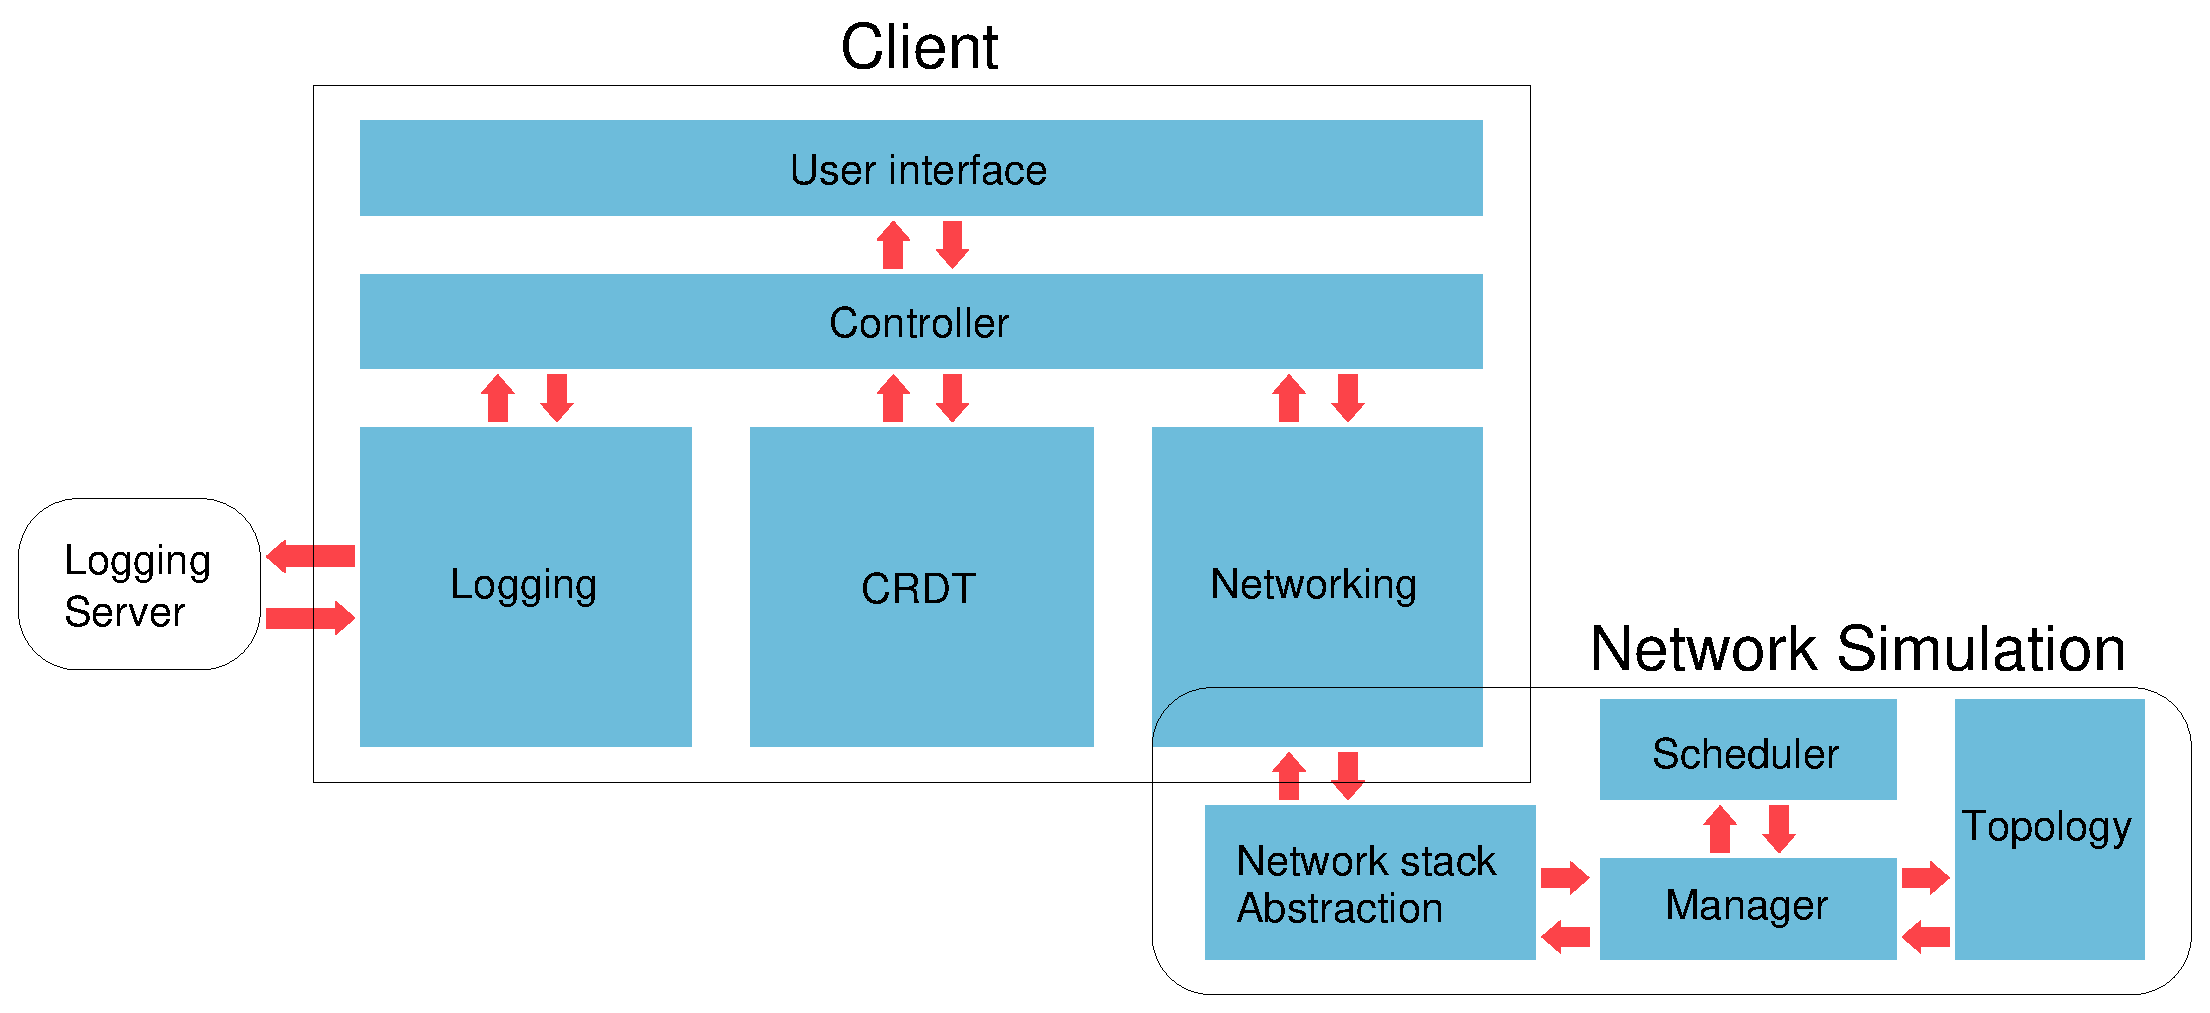
\includegraphics[width=1\linewidth]{figs/sysarch.eps}
		\caption[System Architecture]{An overview of the system architecture implemented for the CRDT-based text editor. Each client has its own UI, controller, CRDT, logger, and networking component. The network module abstracts away the underlying simulation. Many clients can connect to the simulation network abstraction and communicate through it.}
		\label{fig:sysarch}
	\end{figure}
	
	
	\subsection{CRDT}
		To briefly review section [section ref], a text CRDT can be thought of as a set containing characters tagged with totally ordered identifiers. The document is then extracted in full by ordering the elements according to the total order. 
		
		This subsection goes through the structure and capabilities of the CRDT I utilized, how character identifiers are generated and totally ordered, the operations that are supported in the context of text editing, a brief discussion of tombstones left behind by deletions, and some optimizations I added.
		
		\subsubsection{Structure and Functionality}
		In the Related Work section [section ref] various structures were mentioned, such as Treedoc which stores characters in the nodes of a tree and retrieves them in infix order. Rather than using a tree to store characters, my approach implements a singly-linked list. Each link contains exactly a character, a pointer, and is associated with a unique identifier.
		
		The CRDT needs to implement three core methods in order to support text editing
		\begin{enumerate}
			\item \textbf{Insert:} Add a character at a specific index or location
			\item \textbf{Delete:} Remove or mark as deleted any given character
			\item \textbf{Read:} Retrieve the characters in order and return them as a string
		\end{enumerate} 
		
		Inserting characters is done as in standard linked lists -- find the node after which the insert should occur, rewrite its pointer to point to the new node, and repair the broken link with the new node's pointer.
		
		\begin{figure}[htb]
		\centering
		  \begin{tabular}{ >{\centering}m{6cm} >{\centering}m{15mm} >{\centering\arraybackslash}m{6cm} }
		    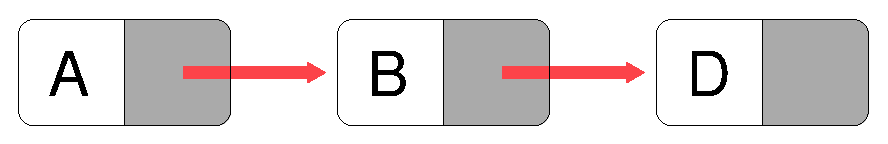
\includegraphics[width=1\linewidth]{figs/linkedlist_0.eps}  &
		    $\longrightarrow$  &
		    \includegraphics[width=1\linewidth]{figs/linkedlist.eps}
		  \end{tabular}
		\caption[Updating linked lists]{A graphical representation of updating linked lists. Here, a new link containing the character `c' is inserted between `b' and `d' to produce `abcd'.}
		\label{fig:linkedlist}
		\end{figure}
		
		Deletes are handled by adding to the relevant link a `deleted' tag. Lastly, the read operation is a linear time traversal over the linked list, beginning with an invisible anchor element that marks the start of the document and cannot be deleted.
		
		Various data structures were considered when implementing this linked list. The most intuitive approach is to implement each link as an instance of a class or structure containing the required identifier, character, and pointer. However, all operations one might want to do on a linked list are $\Theta (n)$: finding a node to insert after or delete requires scanning some proportion of the list. A read is $\Theta (n)$. A much better approach is to implement the linked list within a hash table. Since character identifiers are required to be unique, we can use them as keys in our map and achieve $O(1)$ lookup times [TODO ASSUMPTIONS:Uniform hash, depends on length of key (hash might take time to compute over a string - my strings can grow unbounded as logn) -- BE Precise] for any node. Figure~\ref{fig:hashlist} gives a full CRDT using this structure. Hashing means insert and delete operations can complete in constant time, and only read takes $\Theta (n)$ to retrieve the document.
		
		
		


%\begin{framed}
%	\begin{lstlisting}
%	{
%	 	"0":	{"n":"7.1","c":""},
%		"1.0":	{"c": " ","n":"2.0"},
%		"2.0":	{"c":"w","n":"3.0"},
%		"3.0":	{"c":"o","n":"4.0"},
%		"4.0":	{"c":"r","n":"5.0"},
%		"5.0":	{"c":"l","n":"6.0"},
%		"6.0":	{"c":"d","n":null},
%		"7.1":	{"c":"H","n":"8.1"},
%		"8.1":	{"c":"e","n":"9.1"},
%		"9.1":	{"c":"l","n":"10.1"},
%		"10.1":	{"c":"l","n":"11.1"},
%		"11.1":	{"c":"o","n":"1.0"}
%	}
%	\end{lstlisting}
	\begin{figure}[H]
		\centering
		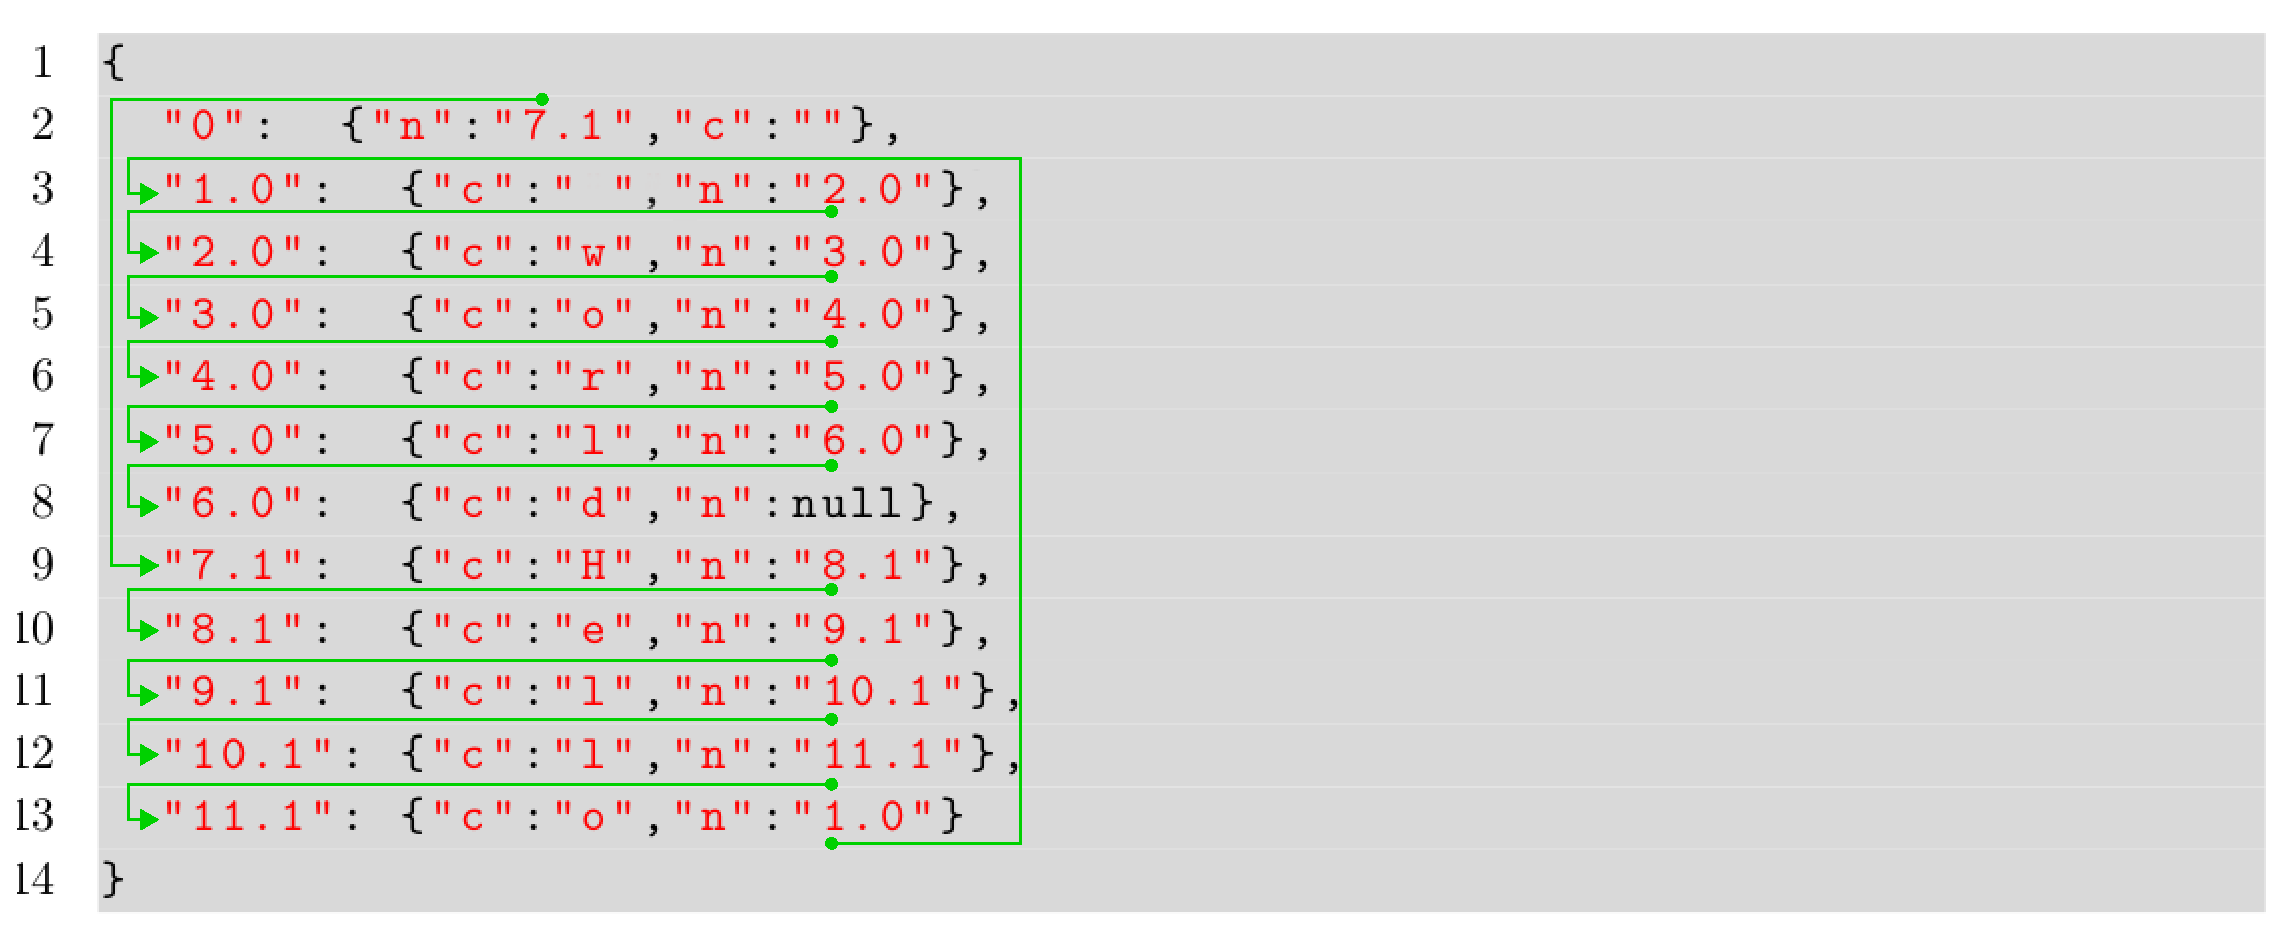
\includegraphics[width=1\linewidth]{figs/hash_list.eps}
		\caption[Annotated CRDT]{A sample CRDT annotated with arrows. These denote the links implemented within the has hash map. The anchor element tagged `0' is invariant and is invisible to the user. The final link, tagged ``6.0'' has no further pointer. The overall string is ``Hello world''.}
		\label{fig:hashlist}
		\end{figure}
%\ end{framed}
		
		Javascript provides two native objects capable of mapping. One is the Map\footnote{\url{https://developer.mozilla.org/en/docs/Web/JavaScript/Reference/Global_Objects/Map}} structure, and another is the standard Javascript Object (referred to as Objects from now on). Both have advantages and disadvantages: Objects only allow strings and numbers to be used as keys, while Maps can use arbitrary entities. On the other hand, Objects serialize very easily to JSON (Javascript Object Notation), while Maps would require their own conversion functions. As we will see in the next section, CRDT keys are pairs of numbers. Thus, the sensible structure would be a Map, as we can map from pairs to values. Unfortunately, Maps natively do not hash the contents of the keys, but only the reference pointing to the key. I implemented both Map and Object variants of the CRDT, but the original pointer to the identifier used is not retained; it is not possible to retrieve the value associated with a given identifier. To solve this issue I serialized the key pair into a string on each lookup and insert (which, being immutable in Javascript are compared by content rather than pointer). At that point Maps have no more advantages over Objects and a distinct disadvantage in terms of serializing to JSON. Thus, I eventually settled on CRDTs implemented using Objects as lookup structures.
		
		From now on, ``CRDT'' and ``linked-list'' will be used interchangeably.
	
		\subsubsection{Identifiers}
		
		Recall that CRDT identifiers are required to be globally unique and totally ordered. My CRDT is advantageous over tree-based CRDTs in that generating identifiers is straightforward. Each client has a unique ID (referred to as \textit{cid}) which forms one part of each identifier. A \textit{cid} can either be randomly generated or provided by the bootstrapping server for the P2P network. In this project, the network simulation provides unique \textit{cid}s.
		
		Define an identifier generated by client $i$ to be a pair $(t_i, cid_i)$ where $t_i$ is a the value of a local counter incremented on every insert. $cid_i$ is the globally unique identifier of the client. Since each client provides a monotonically increasing $t$ per identifier, and $cid$ is globally unique, every pair generated in the system is guaranteed to be unique.
		
		The counter $t_i$ is maintained as a Lamport clock~\cite{lamport1978}. If an incoming operation has a greater $t_j$ than the local clock, the value of $t_i$ is set to $t_j$. This guarantees that any operation that is causally generated after another (defined in more detail later) has a higher clock value, which in turn guarantees that only concurrent operations can have the same clock value. Note that this does not mean all concurrent operations have the same clock value. The only meaningful deduction we can make is that a remote, incoming operation that has a lower $t$ than the local clock, must have been concurrent. This is a key idea utilized when inserting characters concurrently.
		
		We can now define a total order over the identifiers:
		
		\[(t_1, cid_1) < (t_2, cid_2) \Leftrightarrow t_1 < t_2 \lor (t_1 = t_2 \land cid_1 < cid_2)\]
		
		
		\subsubsection{Operations}
		The text CRDT supports two core modifying operations: insert and delete.
		
			\paragraph{Insert}
				Inserting a character into the text document generates an insert operation. An insert operation is stored and transmitted as a bundle.
				
				An insert bundle $B$ contains
				\begin{itemize}
					\item A unique identifier $id$ for the character
					\item The character $char$ itself
					\item The node after which to insert the character denoted $after$. This corresponds to the position in the linked list at which the character needs to be spliced in. $after$ is another unique identifier
				\end{itemize}
			
\vspace{3mm}	
\begin{lstlisting}[caption=Insert Bundle Type Signature]
interface InsertMessage {
    id: string,
    char: string,
    after: string
}
\end{lstlisting}
				
				Incorporating an insert bundle $B$ into the CRDT is the following sequence of steps
				\begin{enumerate}
					\item Locate in the hash table the node $Prev$ corresponding to the $B.after$ identifier
					\item While $Prev.next \geq B.id$, do $Prev = get(Prev.next)$. This skips over local concurrently inserted nodes
					\item Create a new node $Node$, with $Node.char = B.char$ and $Node.next = Prev.next$
					\item Create a new hash table entry with key $B.id$ and value $Node$ $B.id$
					\item Rewrite $Prev.next = B.id$ pointer to point to the new $Node$, repairing the linked list
				\end{enumerate}
				
				This is the standard procedure to insert a new node into a linked list, with the exception of step 2. This is the key step to ensure that all clients converge to the same string, no matter what order the concurrent inserts are incorporated.
				
				To understand the intuition behind why this works, recall the reason for utilizing a Lamport clock: we can deduce that a remote, incoming identifier $id_a$ and some locally generated $id_b$, are concurrent if $id_a \leq id_b$ . Thus, when incorporating $id_a$, we skip over local, concurrent identifiers until finding one where the condition $\leq$ fails and insert there. Reciprocally, once local operations arrive at the sender, the same algorithm will be applied. The arrived operations will have greater identifiers, $id_b > id_a$ (same identifiers of concern as before, just on the other client), and so step 2 will iterate over nothing and insert them before $id_a$. Thus on both clients, $id_a$ will be reside after $id_b$ in the linked list.
				
			\paragraph{Delete}
				Deleting a character from the text document generates a delete operation, which is transmitted as a bundle $B$ containing
				\begin{itemize}
					\item The target character's identifier to be deleted $deleteId$
				\end{itemize}
				
\vspace{3mm}
\begin{lstlisting}[caption=Delete Bundle Type Signature]
interface DeleteMessage {
    deleteId: string
}
\end{lstlisting}				
				
				Incorporating a delete bundle into the CRDT is straightforward
				\begin{enumerate}
					\item Locate the node $N$ corresponding to $B.deleteId$
					\item Set a boolean flag in $N.d$ to true
				\end{enumerate}
				
		\subsection{Tombstones}
			The delete operation described previously never removes nodes, but leaves them behind as tombstones. Some CRDTs, such as Logoot described in section [section ref], are structured such that the document is series of independent nodes, which are arranged solely according to their identifiers. Thus, a node can be fully removed without consequence to other nodes. In my CRDT, each node depends on the prior node in the linked list. Unless we can establish that each client has received and executed a delete operation, we cannot remove our node from the linked list -- other clients may be executing concurrent edits which depend on that node, are working on a document offline, or on a very high latency link.
			
			The process of establishing that each client has received and executed an operation can be achieved using an expensive commitment protocol, which is what is suggested in \cite{preguica2009}. In effect, the system periodically executes a distributed garbage collection. While possible, I have not implemented this protocol. While remove tombstones may be necessary after the data structure becomes too large, until such a point tombstones are useful in implementing undo functionality for the text editor. This is discussed in section [section ref].
			
			[TODO make reference to another section, perhaps after vector clock addition, to garbage collecting the tombstones using the vectors]
		
		\subsection{Optimizations}
			The insert operation produces a bundle which contains exactly one character, one identifier, and one \textit{after} tag. We can drastically cut the number of operations generated, and thus packets sent in the network, by allowing an insert bundle to contain a contiguous sequence of characters. 
			
			An optimized insert bundle contains
			\begin{itemize}
				\item A unique identifier  $(t, cid)$ for the first character
				\item The character sequence $s$ itself
				\item The node after which to insert the character sequence denoted $(t_{after}, c)$
			\end{itemize}
			The receiver CRDT incorporates the bundle by generating a new node for each character $s_i$ with identifier $(t + i, cid)$. The first node is pointed to by the $(t_{after}, c)$ $after$ pointer and each new node points to $(t + (i+1), c)$. The final node points to the original target of $(t_{after}, c$.
			
			This insert optimization has potentially massive gains in terms of network efficiency. With the optimization, at best, an entire document could be inserted at once, sending exactly one identifier plus a string of length $n$ in a single packet. A more likely scenario is word-by-word or line-by-line insertion. At worst, we revert to the unoptimized case: $n$ characters and identifiers are sent in $n$ packets. If we assume the network protocol can send arbitrarily long packets, the application-layer network capacity requirement is reduced to between $\Omega (n)$ and $O(nlog(n))$ from $\Theta(nlog(n))$. Written another way, if an average of $m$ characters is sent per packet, the capacity needed is $\Theta ((m+log(n)) * n/m)$ = $\Theta (n + nlog(n)/m)$. The number of packets is reduced to $\Theta (n/m)$. The reduction in number of packets is desirable since standard protocols such as TCP have high per-packet dissemination overheads.
			
			Another optimization I added was renaming tags and names to be as short as possible (often single characters), so that the resulting serialized JSON string sent over the network is as short as possible. As discussed before [section ref TODO], alternatives to JSON such as Protocol Buffers would eliminate almost all of these overheads, but this would make comparison with ShareJS less fair.
	
	\subsection{Network simulation}

	
		The section describes the network simulation that delivers operation bundles from one client to another. First, I will detail the initial assumptions I made. This is followed by the abstractions the simulation provides to each client. Next I describe the core difficulty in implementing a simulation: the scheduler. Lastly, I will relax the assumptions made to more closely mirror real world situations.
		
		Note that the term \textit{simulation} is not fully correct, as the networking component does not model a real network protocol but is in use to allow analysis and some detail is included, such a specific network topology. An alternative might be \textit{emulation}, as I use implement a replacement for the functionality of a protocol, without implementing the protocol itself. For simplicity I will continue with \textit{simulation}.
		
		\subsubsection{Assumptions} 
		The CRDT I implemented requires that messages be delivered causally~\cite{concdistsystems}. We define the happens-before relation \(a \rightarrow b\) to be true whenever $a$ happens before $b$ on the same process, for example \[Receive\ Insert\ ``Hello'' \rightarrow Insert\ `` World''\]
		We then require that all events ordered by $\rightarrow$ be delivered in a valid ordering according to $\rightarrow$. We call this ``Causal Order''. This defines a partial order, since there may be some $A$ and $B$ such that neither $A \rightarrow B$ nor $B \rightarrow A$ holds. Concurrent operations can be delivered in any order since they are guaranteed to commute by the properties of the CRDT.
		
		To justify the causal order delivery requirement, simply take the case of inserting a link into a linked list after a node that does not exist yet. In the CRDT, the links embed the causal ordering thus we require causal delivery.
		
		\underline{Network Assumptions}. These are guaranteed by the simulation.
		\begin{enumerate}
			\item Unchanging network topology
			\item In order delivery on any single link in the network
			\item No packets are lost
		\end{enumerate}
		
		Along with this, my implementation of individual clients guarantees:
		\begin{enumerate}
			\item Received packets are forwarded in order, i.e. if $A$ arrives before $B$, then $A$ is forwarded before $B$.
			\item Received packets are broadcast to peers before the client generates and broadcasts potentially dependent operations.
		\end{enumerate} 
		
		The simulation and client guarantees provide causal delivery.
		
		\begin{proof}[Guarantee of Causal Delivery]
		
		Assume there is some packet $A$ in the network. A packet $B$ is sent in a causally dependent manner, i.e. $A \rightarrow B$, thus $B$ must be delivered after $A$ on every client in the network. Denote the network node which generated $B$ as $sender_B$.
		
		Proof by induction on any shortest path $p$ from $sender_B$ to another node on $p$. Denote the $i$\textsuperscript{th} node on $p$ as $p_i$. Use $i$ as the induction variable. The broadcast dispersal mechanism used in the simulation delivers packets to every node via the shortest path from a sender as long as the network is static and no packets are lost, which are guaranteed by network assumptions 1 and 3.
		
		Base case, $i = 1$.\\
		As $p_1$ is exactly one hop from $sender_B$, and $sender_B$ must have put the packets onto the link in order by client assumption 2, and packets are delivered in order over any link, $p_1$ must receive the packets in order.
		
		Inductive case, $i = m$.\\
		Assume $p_m$ receives packet $A$, then $B$ i.e. in order. By client assumption 1 -- in order forwarding --, and network assumption 2 -- in order delivery on individual links --, node $p_{m+1}$ must receive $A$ followed by $B$. Because $p_{m+1}$ lies on the shortest path, it cannot have received the packets before.
		
		Thus, the network guarantees causally ordered delivery to every node in the network.
		
		
		
%		\begin{proof}[Guarantee of Causal Delivery]
%			Part 1. Assume a single packet $A$ is in the network. In order to generate a second packet $B$ such that $A \rightarrow B$, a client must have received $A$, then sent a packet $B$. This process must send $A$ followed by $B$ to all neighbors by client guarantee 2. Thus causally dependent packets are guaranteed to be sent in order initially.
	%		
%			Part 2. Proof by contradiction.
	%		
%			Assume that at some point in the network, a client receives: $B$ before $A$. Also assume and that $A \rightarrow B$. By Part 1, if $A \rightarrow B$, it must initially have been that $A$ was sent before $B$. This means $B$ overtook $A$ at some point. So, one of the following must have occurred:
	%		
%			The packets were delivered out of order on a single link. This cannot happen by assumption 2 of the network guarantees.
	%		
%			$A$ was lost on a link, $B$ was delivered, and $A$ arrived on a different route. This cannot happen by assumption 3 of the network guarantees.
	%		
%			The topology changed between a client forwarded $A$ and $B$ such that $B$ took a faster route than $A$. This cannot happen by assumption 1 of the network guarantees.
%			
%			A client forwarded $B$ before $A$. This cannot happen by assumption 1 of the client guarantees.
%			
%			All possible ways $B$ could overtake $A$ have been contradicted. Thus, the original assumption must be false. And $B$ can never be received before $A$.
			
			
		 
			
		
			%Proof by contradiction. Assume a client receives some packets $A$ and $B$ and that at some prior point, it must have been the case that $A \rightarrow B$. This implies that somewhere in the network $A$ and $B$ switched order. However, on any individual link, $A$ and $B$ stay in order by network assumption 2 above. At any node, packets cannot switch order either, since the implementation immediately forwards an incoming packet to its neighbors (If a particular client generated $B$, it is put on a link after $A$ by the same condition). Lastly, because the network does not change topology and the protocol is deterministic flooding, packets do not dynamically adjust routes and so any packet that begins in order $A$, then $B$ stays in order $A$, $B$. Thus, in no case can $A$ and $B$ switch order and our assumption must be incorrect. Either $A \rightarrow B$ or it must have been the case that $A \not\rightarrow B$ to begin with. The first case proves our goal and the second is irrelevant.
		\end{proof}
		
		That the network is able to guarantee causal delivery is a strong assumption and cannot be made in general. We will see in section [section ref] how to relax network assumptions 1 and 2.
		
		\subsubsection{Abstraction}
		My network simulation is implemented in two parts: a manager which is shared between all simulated clients, and a Network Interface, of which each client has a copy. The Network Interface essentially emulates the top of a classic network stack, whereas the manager abstracts away the bottom layers. 

		\paragraph{Network Interface} The essential parts of the Network Interface type signature are shown below.
		
\begin{lstlisting}[caption=NetworkInterface Type Signature (cleaned)]
interface NetworkInterface {
	isEnabled: () => boolean;
	enable: () => void;
	setClientId: (ClientId) => void;
	setManager: (NetworkManager) => void;
	requestCRDT: (ClientId) => void;
	returnCRDT: (ClientId, MapCRDTStore) => void;
	broadcast: (PreparedPacket) => void;
	receive: (NetworkPacket) => void;
}
\end{lstlisting}

		The primary mechanism for disseminating a packet to other clients is via the \lstinline|NetworkInterface.broadcast| method, which in turn calls the \lstinline|broadcast| method of the \lstinline|NetworkManager| (see [section ref]). It accepts a \lstinline|PreparedPacket| which is an object that contains a bundle (such as \lstinline|InsertMessage| or \lstinline|DeleteMessage| from section [section ref]) and a tag which the receiver uses to disambiguate the type of the incoming packet. This is required since packets are serialized to strings when sent over the network and all type information is lost in the process.
\begin{lstlisting}	
interface PreparedPacket {
	type: "i" | "d" | "reqCRDT" | "retCRDT",    // insert or delete message, or request CRDT or return CRDT
	bundle: CRDTTypes.InsertMessage | CRDTTypes.DeleteMessage | RequestCRDTMessage | ReturnCRDTMessage;
}
\end{lstlisting}
		
		Other types of bundles that can be sent are \lstinline|RequestCRDTMessage| and \lstinline|ReturnCRDTMessage|. These are special messages which clients use when joining the network and requesting a copy of the CRDT be sent from an active client.
		
		\paragraph{Joining the Network}
		During the execution of a simulation, clients may join the network (but not leave) at any time. Only the first client gets to create a new CRDT. Any other client must request a copy of that CRDT when joining via \lstinline|RequestCRDTMessage|. This means that there is at least 1 round trip time before a new editor can come online. The \lstinline|ReturnCRDTMessage|s become quite large -- the later a client joins, the larger the CRDT, and the larger the packet. However, they would also have avoided many individual packets being delivered to them in the meantime.
		
		An alternative method to requesting an up-to-date CRDT is to begin with a empty CRDT and replay all subsequent operations on it. This would however be even less efficient as it would require all remote clients to store all of their previous operations forever (or have a server store them), and the local client would have to spend computational time reintegrating all the changes. The downside to obtaining an up to date copy is that there is no straightforward way to do a partial replay. If a client simply has an out of date CRDT, it must request an entire new copy as if rejoining the network.
		
		At this point it is important to acknowledge that introducing dynamic network joining violates one of the guarantees of [section ref]. Namely, incorporating new clients over time changes the network topology and thus the guarantee of causal delivery no longer holds. The introduction of vector clocks [section ref] will restore this guarantee.
		
		\paragraph{Network Manager}
		The lower layers of the network stack are provided by the Network Manager. It has two key methods: \lstinline|NetworkManager.transmit(sender, packet)| and \lstinline|NetworkManager.unicast(from, to, packet)|. The simulation is given a predefined topology, which contains connectivity and latency information (discussed further in section [section ref]). Thus, when a client's \lstinline|NetworkInterface| calls \lstinline|NetworkManager.broadcast|, the manager knows which clients are neighbors and corresponding link latencies, and can schedule a delivery event for each. The \lstinline|NetworkManager.unicast| is used for point to point, single hop communication when joining the network and requesting or sending copies of CRDTs. Overall, this module replaces the network and data layer of most network stacks and abstracts away how packets get exchanged between neighboring clients.
		
		
		\subsubsection{Scheduler}
		Although this subsection falls under the Network Simulation section of this document, the scheduler is an altogether more general driver of the simulation. However, its main task during an experiment is to deliver packets between nodes, which is why it is listed here.
		
		A simulation scheduler is responsible for mutating system state, based on events given to it to be executed at specific times. To schedule an event, an object needs to call the \lstinline|Scheduler.addEvent| method, which is listed below.
\begin{lstlisting}[caption=The Scheduler.addEvent method]
public addEvent(time: number, clock: number, action: any) {
    let heapElem: DualKeyHeapElement = {
        pKey: time,
        sKey: clock,
        payload: action
    };
    this.heap.insert(heapElem);
}
\end{lstlisting}

		My scheduler is somewhat more sophisticated than might be expected in that it takes two keys for scheduling: a primary key $pKey$, and a secondary key $sKey$. The need for this arose when submitting multiple packets from a single client at the same time - the original underlying data structure, a heap with a single key, makes no first-in first-out assurances. Thus, packets on a link could arrive out of order, which violated one of the guarantees the network has to provide [reference needed]. To fix this, my scheduler breaks ties using $sKey$, which is a monotonically increasing counter provided by the caller.
		
		The key property of a correct scheduler, as noted in the Part II Computer Systems Modeling \cite[slide 120]{compsysmodeling} course, is that the next executed event be the one with the least remaining time. To do this efficiently, I implemented a heap that orders elements based on the two keys discussed above. Using a heap, we get $\Theta (log(n))$ retrieval per element.
		
		When the simulation is running, the scheduler removes the top event $E$ off the heap, decreases all remaining events' primary keys by $E.pKey$, and executes $E.payload$. This may in turn generate more events which are added back into the heap. The scheduler continues this until paused or the event queue is empty.
		
		Because the simulation needs to be seeded with events and simulated action in order to do anything useful, before letting the execution begin, the scheduler is also used to add a set of mock insert and delete events, which together constitute an experiment. This is discussed in more detail in [section ref]. Once running, its primary use is delivering packets.
		
		\paragraph{Time}
		The concept of time in a simulation is generally taken to be ``logical time''. The system begins in $t = 0$, and each subsequent event moves the $t$ variable forward. This works perfectly well for the CRDT-based system, since the latency on any individual network link is well defined and known.
		
		The alternative `time' that can be used is real time. The amount of time until some next event is given in milliseconds to wait, rather than a logical delta which is skipped over. Using this concept of time in a simulation introduces extra complexity, primarily stemming from inaccuracy in timers provided by the host platform. Indeed, it is likely that some events will have very small deltas, for which starting and stopping a timer would be impossible. To handle this difficulty, the scheduler runs, in order, all ready events whenever it wakes up rather than just one at a time.
		
		In this project, I implemented both an event-driven scheduler and a timer-driven scheduler. The timer-driven version is useful when debugging and watching the simulation unfold in real time, whereas the event-driven version runs as fast as the hardware lets it. However, I found that I could, to an extent, emulate the timer-driven scheduler using the event-driven scheduler by adding a sleep proportional to the $\Delta t$ until the next event. As the event-driven version is more flexible, and simpler -- the driver is simple while loop, rather than recursively set timers with callbacks -- I decided to use it when executing experiments on the CRDT-based system.
		
		Luckily, the timer-driven scheduler is useful in the comparative system. In it, packets are actually delivered via sockets and the operating system, which means that logical time can no longer be used. This is discussed further in section [section ref].
		
		
		\subsubsection{Causal Delivery}
		Until this point, the network has guaranteed causal delivery of packets based on very strong assumptions and knowledge of the system implementation [reference needed]. We can relax these to allow out of order delivery and a changing network topology without a specific implementation. This can be done by ensuring causal delivery using vector clocks \cite{fidge1987}.
		
		In addition to the two part network stack, there is now an additional layer between a client and the network interface. We make a distinction between receiving and delivering a message. Receiving is the arrival of a message at a client, whereas delivery is the step of passing the message from the network stack to the application itself. Causal delivery guarantees that messages are delivered such that $A \rightarrow B \Rightarrow\ deliver(A)$, $deliver(B)$.
		
				
	\begin{figure}[H]
	\centering
	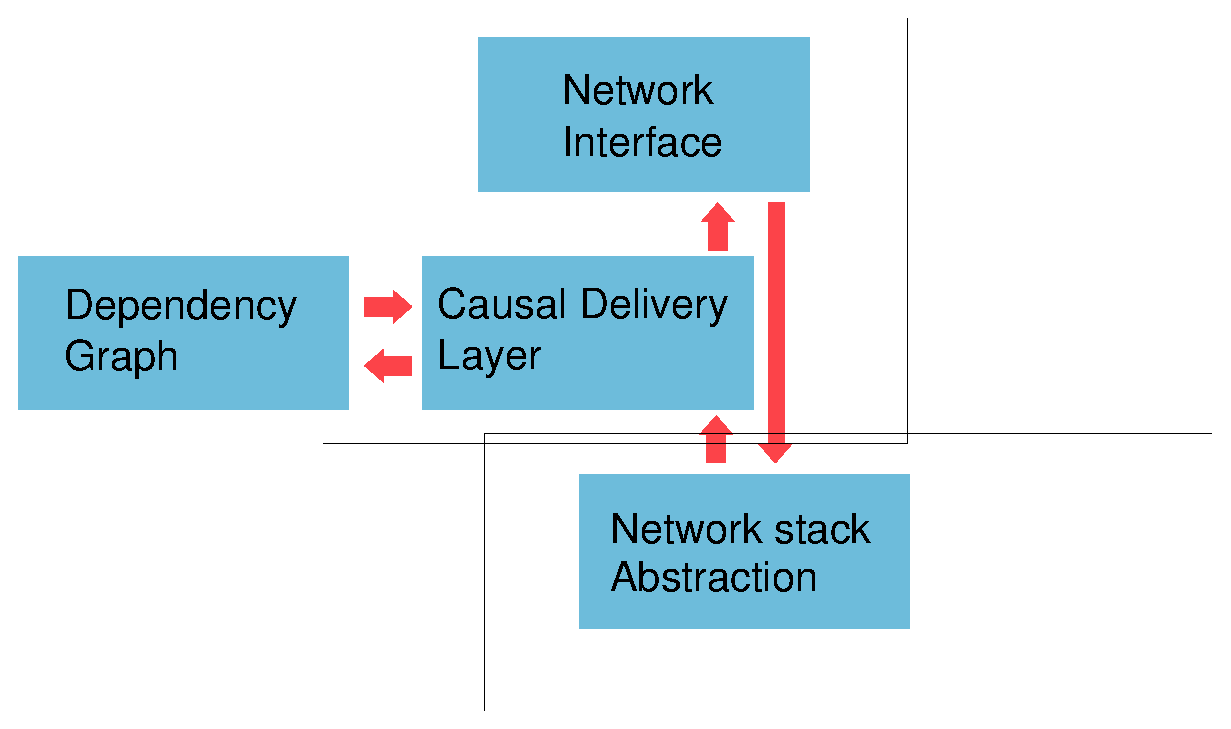
\includegraphics[width=1\linewidth]{figs/causal_arch.eps}
	\caption[Ensuring Causal Delivery]{}
	\label{fig:causal}
	\end{figure}

		
		\paragraph{Vector Clocks}
		A vector clock is an list of sequence numbers, one per distributed process. At the time the system is initialized, all clients have a vector of zeros. According to the original paper by Fidge, there are 5 rules for updating which ensure that causal order can be determined by comparing vectors. The specifics of vector clocks are outlined in Appendix~\ref{appendix:vectorclocks}. The properties of vector clocks guarantee that \[ A \rightarrow B\ \Leftrightarrow Vector(A) < Vector(B)\] where $<$ is defined to in the appendix.
		
		Fidge's nth[TODO] rule indicates that a receiver should increment its own local clock value on receipt of a message, as well as on sending its own messages. While this rule makes it easy to determine whether a message comes before or after or occurred concurrently with another, it is not so straightforward to determine, for instance, if a message overtook another on the same link, or how many messages occurred between two given vectors.
		
		\paragraph{Modified Vector Clocks}
		Causal delivery layers delay messages that arrive before all of their causal dependencies are delivered. This requires calculating exactly which messages are missing, before a delayed message can be passed from the buffer to the client.
		
		To do this simply, I modified the rule of incrementing local clocks on receipt, and only increment locally whenever a message is generated. This way, each value in a vector represents exactly how many messages have been sent by the corresponding client. This avoids conflating `how many messages this client has seen' with `how many messages this client has generated'.
		
		We can now determine concurrent, causally dependent and causally prior messages by comparing vectors. We define the latter two about $<$.
		
		Concurrent. Given two vectors $v1$ and $v2$, they occurred concurrently iff \[\exists c,c' \in v1,\ v2.\ v1.c > v2.c\ \land\ v1.c' > v2.c'\]
		
		Causally Dependent and Causally Prior. Given vectors $v1$ and $v2$, \[v1\ <\ v2 \iff\ \forall c \in v1, v2.\ v1.c \leq v2.c\ \land\ \exists c' \in v1, v2.\ v1.c' < v2.c'\]
		In this definition, $v2$ is causally dependent on $v1$ and $v1$ is causally prior to $v2$.
		
		If a client receives a vector $v$ that is concurrent with the client's current vector $s$, the causal network layer immediately delivers the message to the client. If $v < s$, then the message has been seen before and can be discarded. In the case that $s < v$, the Delta Vector can be computed.
		
		A Delta Vector $dv$ between $v1$ and $v2$ is their element-wise difference. If the sizes of the vectors mismatch, treat the missing vector elements as being equal to 0. Delta vectors are useful for delivering messages efficiently.
		
		
		\paragraph{Efficient Delivery}
		The causal delivery middleware must buffer all messages with dependencies that have not arrived yet. This means, that on each new message, the buffer must be searched for messages that can be delivered. This could lead to a cascade of deliveries which if implemented naiively is quadratic in the number of buffered messages.
		
		Instead, using Delta Vectors we can form a dependency graph which allows more efficient delivery.
		
		\begin{figure}[H]
		\centering
		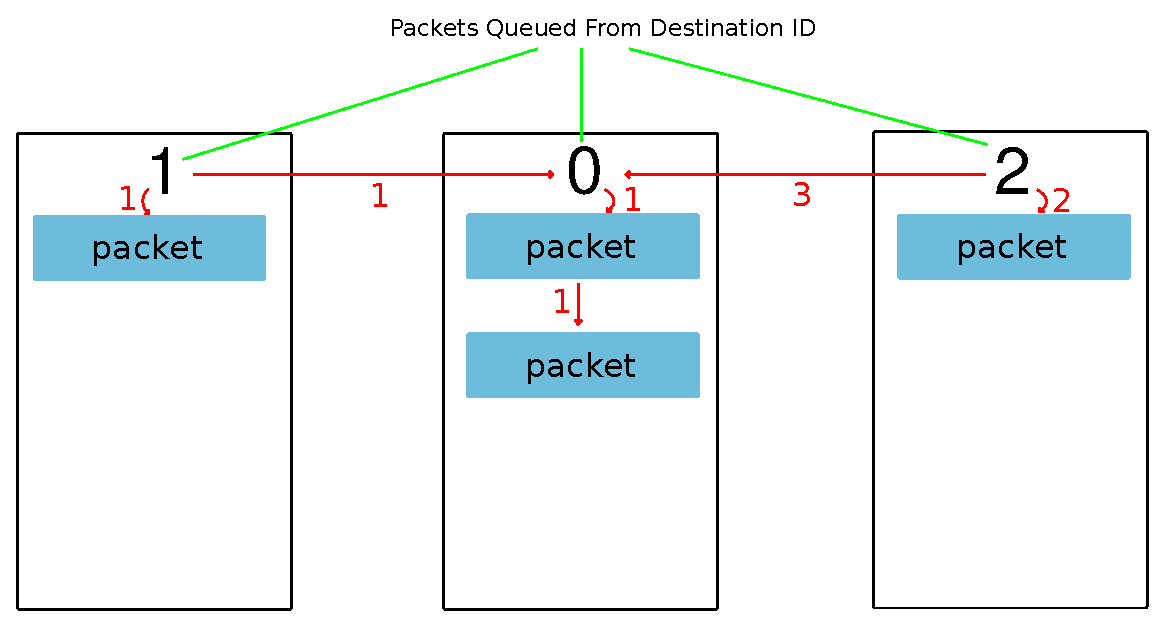
\includegraphics[width=1\linewidth]{figs/efficient_message_buffer.eps}
		\caption[Dependency Graph in Message Buffer]{A representation of the graph structure used to efficiently deliver packets. When a new packet arrives from some destination D, all outgoing links from D are decremented. The target of each link checks the head of its queue for potential delivery. The efficiency gain relies on the fact that messages from the same client must be delivered sequentially.}
		\label{fig:efficient}
		\end{figure}
	
	
\section{ShareJS Comparative Environment}

	The main difficulty when building a ShareJS-based comparative system is adapting it to allow executing the same format experiments as the system built bottom up before. The main components in enabling this were incorporating the real-time scheduler discussed in [section ref], and inserting log statements to record data to the logging server.
	
	\paragraph{Scheduling}
	An experiment consists, at its most basic, of a set of simulated events that each client performs at given times. In the CRDT system, these events could be scheduled in logical time, as the entire simulation was under the control of the same system and all event times and durations were deterministic. Here, ShareJS requires that sockets be used to transmit operations between clients, even if they are all on the same machine. Nondeterminism is introduced by going through a traditional networking stack, so logical time is no longer applicable.
	
	The real-time scheduler takes the basic time unit to be a millisecond, and executes experiment events accordingly. Of course, this choice of unit is arbitrary and can be sped up or slowed down by a constant multiplier. The unchanging factor is the time needed to deliver packets via a real network stack using TCP (the standard protocol used by ShareJS). It makes sense to schedule events on the same order of magnitude as a network round trip time: much less, and all events occur nearly instantaneously and concurrently on all clients. Much slower, and there is little concurrency to explore. Thus a middle ground, similar to the average link latency, is the best choice when designing experiments. This core idea is used when automatic the creation of experiments [section ref].
	
	\paragraph{Logging}
	Enabling data logging primarily consists of inserting log lines at critical points that reveal interesting information about the system. The most important of these are the receiving or sending of any packets from a client or the server, and total memory consumption of the clients before and after the simulation. This was done by reading the ShareJS source code and inserting references to a global logging class at the appropriate points.
	
\section{Experiment Creation and Use}

	This section deals with the creation and analysis of the experiments. First I outline the overall system work flow. Then, I discuss the design of an individual experiment. Lastly, I examine why I decided to log to text files, then separately parse and analyze these files.

	\subsection{Work Flow}
	On the whole, this project operates as in Figure~\ref{fig:workflow}. 
	
	\begin{figure}[htb]
	\centering
	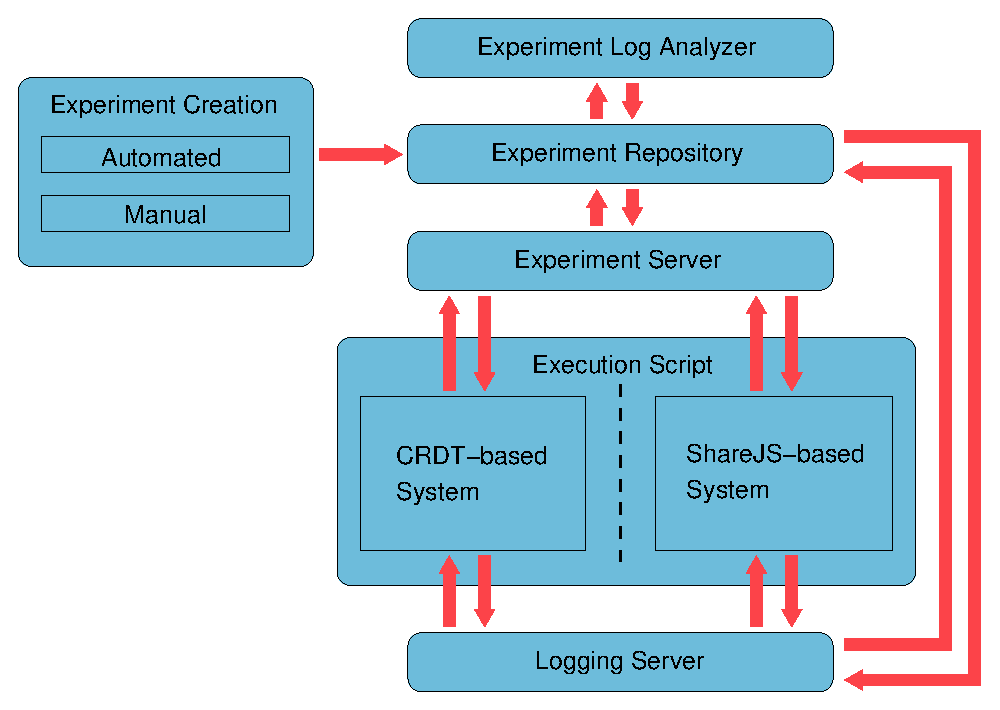
\includegraphics[width=1\linewidth]{figs/workflow.eps}
	\caption[Workflow]{}
	\label{fig:workflow}
	\end{figure}

	
	
	Manually or with a custom script, experiment setup files are created, with specifications over which variations should be executed (such as different topologies or optimizations enabled). An experiment server provides whichever experiment and variant is queued to the requester, which may be the CRDT-based system, or the ShareJS-based one. In either case, the same basic data is served, though the experiment variations only apply to the CRDT-based system. The system then runs the experiment and submits the resulting log back to a logging server that then identifies which experiment was served, and writes the log to the correct file system directory. Then at some future point, a separate script collects logs and summarizes them into digestible formats.

	\subsection{Experiment Design}
	
	A basic experiment must specify the number of clients participating and when they join the network, a set of events for each client to execute, and the network topology and link latencies. I chose to save this data in a JSON file which is easily served from an experiment server to the web browser (browsers do not have facilities for automatically accessing local files for security reasons, otherwise the server would be redundant). Other options in experiment setups are variants, such as different network topologies to run the same experiment on and the type of scheduler to use in the CRDT-based system.	Listing~\ref{lst:simple} below makes all of these features visible for a simple experiment.
	

\begin{lstlisting}[caption={A simple JSON experiment setup. Comments added for explanation and not part of JSON syntax}, label={lst:simple}]
{
	// Experiment Name
    "experiment_name": "experiment_1", 	
	// How many clients and when they join
    "clients": [0,0,0],		
	// CRDT-only: Per client values used to compute link latencies	
    "network": {				
        "0": {"latency": 196.7632081023716}, 
        "1": {"latency": 220.01040150077455}, 
        "2": {"latency": 122.31541467483453}
    },
	// CRDT-only: type of scheduler to use
    "execution": "event-driven", 	
	// Scheduled events
    "events": {						
        "0": {					// Events for client 0
         "insert": {				// Insert events for client 0
                "0": {				// Insert "coliseums" at time 0, index 0
                    "chars": "coliseums", 
                    "after": 0
                }
            }, 
            "delete": {}			// No delete events
        }, 
        "1": {					// Events for client 1
            "insert": {				// Insert events for client 1
                "15": {				// Insert "tackling" at time 15, index 0
                    "chars": "tackling", 		
                    "after": 0
                }
            }, 
            "delete": {}			// No delete events
        }, 
        "2": {					// Events for client 1
            "insert": {				// Insert events for client 1
                "30": {				// Insert "freshening" at time 30, index 0
                    "chars": "freshening", 
                    "after": 0
                }
            }, 
            "delete": {}			// No delete events
        }
	},
	// CRDT-only: Topologies over which to run the same experiment
    "topology": [					
        "fully-connected", 
        "star"
    ]
}
\end{lstlisting}

	The choice to assign latencies per-node, and calculate a link latency as the average between two nodes' values, rather than assign per-link stems from the need to have one network description that fits any topology. It also models the real world better on a conceptual level: a device with one high latency link, such as a mobile phone, will likely have only higher latency links rather than some fast and slow links. This ``higher on all connections'' is modeled with the average between a (high-valued) node and its neighbors.

	
	\subsection{Separation of Concerns}
	
	A major decision that was made was to separate log analysis from the system generating the log itself. One reason for this was that it is good software engineering: one component should do one task. Another is that a separate analysis layer can analyze results from both the ShareJS and CRDT systems, rather than duplicating functionality for each system. On the other hand, modules for examining logged packet departures and arrivals end up resembling a set of `clients', much like the original simulations' and ShareJS's clients. However, I decided that having a system common to both that is separate and easily extensible is worth duplicating some high level functionality. The result is a Python script which parses and summarizes multiple log files from a single experiment.
	
	The analyzer pairs up send and receive log lines for each packet and calculates link latencies (important for ShareJS where latencies are nondeterministic) and length of packets, records the increases in memory usage at checkpoints in the log files, and various other statistics. A sample output is listed in Appendix~\ref{appendix:simplelogsummary}.	
	
	
	
\section{Extension: Local Undo}
	
	In interactive systems undo and redo are key features \cite{shneiderman1982}. As such, it is an interesting extension to the capabilities of a CRDT beyond basic insertion and deletion. I chose to implement a local undo -- that is, only allow undoing and redoing operations that were performed locally -- rather than a global undo, where everyone can modify any operation, at the suggestion of my supervisor. The approaches detailed below were developed originally prior to reading related literature, but one is very similar to that of Logoot Undo [section ref needed].
	
	\subsection{Overview}
	Each client keeps a local stack of operations that it produced. The stack can be truncated to a certain length to avoid ever-growing memory consumption. When undoing an operation, a pointer is moved back down the stack and the inverse operation of the corresponding item on the stack is generated and broadcast to other clients.
	
	There are two operations that can be undone or redone: insert and delete. Only one client can ever locally generate an insert event (as each character is tagged with a globally unique identifier generated on the client) and thus it can undo and redo the operation. In the other case, two clients can concurrently delete the same character and so have the same operation on their local stack. How undoing and redoing this concurrent case is handled leads to two different semantics and consistency models. However, the insert is handled the same way in both cases.
	
	
	\subsection{Insert}
	The undoing of an insert can be thought of as a deletion, but this leads to the idea undo/redo can be implemented using the existing delete and insert operations. However, this is not feasible: doing a `redo insert' by inserting a new character of the same value, is not the same thing as redoing the insertion of the original character -- this is especially obvious when looking at the structure of the CRDT. Since each character is identified uniquely, the redo must reintroduce the same character with the same unique identifier rather than creating a new one with a fresh tag. Additionally, other clients may have performed concurrent operations on the character which must be brought back into effect on redo. The solution to this is discussed in the following subsections.
	
		\subsubsection{Undo/Redo Insert Semantics}
		The creator of an insert can choose to undo its creation at any point in time. To satisfy the CCI consistency model and semantics (defined in [section ref] and below), an undo and a redo should have \textit{the same effect on the visible text as if the prior creation or undo never occurred}. For instance, if $A$ creates a character which is deleted by $B$, and the creation is undone and then redone by $A$, the character should still not be visible: the effect of client $B$s delete come back into effect as if $A$ never undid the insertion.
		
		Using this idea, it is evident that `undo insert' and `delete' operations need to be kept separate. Additionally, the operation needs to take precedence over deletions that have occurred subsequently. This along with the fact that a redo needs to reintroduce the original character leads to an effective semantics and straightforward implementation.
		
		\subsubsection{Implementation}
		
		To achieve the desired functionality, I augmented links in the CRDT with an extra boolean `visible' tag (denoted $v$). The two new bundles that need to be created are undo-insert and redo-insert, but these along with the undo-delete and redo-delete bundles (to be seen) all have the same functional form.
		 
		The bundle contains
		\begin{itemize}
			\item The unique identifier of the character to be operated upon
		\end{itemize}
		
		Undo packets also contain, besides the bundle, a string disambiguator to differentiate undo/redo and insert/delete.
		
		The effect of a undo insert packet on CRDT node $L$ is to set $L.v = false$, while a redo insert packet sets $L.v = true$. When the string is queried from the CRDT (i.e. the CRDT `read()' method is called), nodes which have $v = false$ are ignored and not retrieved.
		
		Normally, operations on the same piece of data in a CRDT need to commute. However, in this case, only one client can generate the messages and so conflict from different clients cannot occur. This also means the operations are all causally related by $\rightarrow$, and since the network layer guarantees causal delivery, there is never conflict. Thus, no proof of commutativity is required.
		
	\subsection{Delete}
		Undoing a delete, as mentioned before, is tricker than an insert as multiple clients can perform and therefore `own' a delete at the same time. How this concurrency is handled determines system behavior. The two possibilities are implementing the CCI consistency model and a variant I termed ``Immediate Undo''.
		
		\subsubsection{CCI Undo}
		According to CCI, undoing an delete should lead the system to behave as if the delete never occurred. So, if users 1 and 2 concurrently delete a character, then 1 undoes its removal, the expected result is that the system behaves as if only the 2's delete happened. While this sounds sensible, it is uncomfortable to user 1: they undid their deletion and expect the character to return. In effect, this consistency model requires full consensus between $n$ clients that concurrently deleted a character to return it.
		
			\paragraph{Modified Links}
			While consensus is awkward, it is effectively implemented with counters. The key change is to modify the `deleted' tag of links in the CRDT from boolean to integer.
			
\begin{lstlisting}[caption={New Type Signature of a Link in the CRDT}, mathescape=true]
export interface MapEntry {
	c: string,   // character
	n: string,   // next link
	d?: number,  // (optional) deleted, nonexistant $\Rightarrow$ not deleted
	v?: boolean  // (optional) visible, nonexistant $\Rightarrow$ visible
}
\end{lstlisting}

			\paragraph{Delete, Undo, Redo}
			The first delete bundle can no longer have the effect of setting the boolean `deleted' flag. Instead, on each client it increments the $d$ value in the target link. A redo delete operation will also increment the `deleted' value on every client.
			
			On the other hand, an undo delete operation is a bundle containing only the target ID to undo the deletion of. Its effect on any client is to decrement the `deleted' value.
			
			Now, when the $read()$ method is called on the CRDT, we only retrieve links that satisfy
			
				\[\forall Links\ l.\  (\lnot\exists l.v \lor l.v = true) \land (\lnot\exists l.d \lor l.d = 0 ) \] 
			
			\paragraph{Proof of Commutativity of Delete, Undo, Redo}
			We only need to consider commutativity with other operations that may operate on the same data in the CRDT and therefore conflict. Since any given delete, undo, or redo operation $op$ only affects the specific node $node$ in the linked list identified by $op.deleteId$, the only conflicting operations might be other delete, undo delete, and redo delete operations.
			
			\begin{proof}
				We treat delete and redo delete operations identically, that is having the effect of incrementing $node.d$. An undo delete has the effect of decrementing $node.d$. Any set of these operations applies a sequence of $+1$ and $-1$ to $node.d$. By the commutativity of addition and subtraction, these arithmetic operations can occur in any order, so the delete, undo and redo operations can occur in any order.
			\end{proof}
			
			\paragraph{Cost and Causality}
			TODO
			talk about cost (minimal) and the fact that an undo that happened a long time ago and is no longer on an operation stack has the same weight as one that happened more recently and is still in a stack(by $\rightarrow$) ??? 
			
		\subsubsection{Immediate Undo}
		The CCI Undo is awkward in that it requires consensus to make concurrently deleted characters reappear. It would be preferable for any user to be able to immediately undo a character they may or may not have deleted concurrently with another user.
		
			\paragraph{Semantics}
			To this end, the following describes the desired semantics:
			
			In the case of conflicting concurrent \textit{make-invisible} operations (such as delete or redo delete) and \textit{make-visible} operations (such as undo delete), the \textit{make-visible} operation will take effect.
			
			The follows the idea that a user recalling a prior character likely wishes to utilize it, while a user wishing to remove a character does not care about its presence or absence. Note that this effectively inverts the consensus of CCI Undo to require full concurrent agreement to remove a character.  [talk about no longer having the pitfall of losing an undo/redo in the op stack when it is overwritten]
			
			\paragraph{Implementation}
			In order to support an immediate undo effectively, we need to be able to compare the ``time'' at which a deletion, undo, or redo occurred in order to detect concurrency. Vector clocks allow exactly this. Thus, every such operation needs to tag the data in the CRDT with the vector clock value it occurred at. Then, when other operations arrive which affect the same data, the packet's vector and the vector in the CRDT can be compared and acted upon.
			
			The required modification in the CRDT is that the `deleted' tag of a link $l.d$ now represents a pair ($true/false$, $vector$). The first value is a boolean for whether or not the character is deleted. The second is the vector of the packet that delivered the operation (this cheats a little and reaches across network layers into the causal delivery mechanism to obtain a copy, but is more efficient than redundantly sending the vector both in the bundle and in the packet containing the bundle).
			
			As before, delete, undo delete and redo delete bundles contain only the identifier of the link $l$ to act upon. In non-concurrent cases, that is, operations are causally dependent, the latest operation is applied to $l$. 
			
			If a remote delete or redo delete operation is concurrent with the vector stored in $l.d[1]$, do nothing. This ensures that a local make-visible operation retains its effect (e.g. a undo delete). Otherwise, a make-invisible operation is already in effect and $l.d[0]$ is already $true$.
			
			Similarly, if a remote undo delete operation is concurrent with the vector stored in $l.d[1]$, always set $l.d$ to $false$, so that the make-visible operation takes effect.
			
			In any case, the vector stored at $l.d[1]$ is updated to the current client vector clock.
			
			When the CRDT $read()$ method is called, we only retrieve links that satisfy
			
					\[\forall Links\ l.\  (\lnot\exists l.v \lor l.v = true) \land (\lnot\exists l.d \lor \lnot l.d[0]) \] 
						
			
			\paragraph{Proof of Commutativity}
			
			We only need to consider commutativity with other operations that may operate on the same data in the CRDT and therefore conflict. Since any given delete, undo, or redo operation $op$ only affects the specific node $node$ in the linked list identified by $op.deleteId$, the only conflicting operations might be other delete, undo delete, and redo delete operations.
						
			\begin{proof}
				We treat delete and redo delete operations identically. Any non-concurrent modifications are not considered as the latest causally dependent operation is defined to take effect.
				
				Take a system which begins in quiescence, submits concurrent operations and returns to quiescence. There are three possible cases: delete-delete, delete and delete-undo, and undo-undo.
				
				In the delete-delete scenario, the operations are idempotent: both set $node.d[0]$ to $true$ and $node.d[1]$ to the merged vectors of the two operations. Thus on any client, the target node is no longer visible. The undo-undo case is exactly analogous except $node.d[0] = false$. 
				
				In the delete, delete-undo case (which is one client deletes while another deletes then undoes immediately), any client receiving a single delete $op_{d_1}$ first will set $node.d[0] = true$ and record the current vector in $node.d[1]$. On delivery of the concurrent delete $op_{d_2}$, only the vector at $node.d[1]$ is updated as the node is already marked as deleted. Then, undo $op_{undo_2}$, since it is a \textit{make-visible} operation, and determined to concurrent with the merged vector stored at $node.d[1]$, takes effect and $node.d[0]$ is set to $false$. If $op_{d_2}$ were delivered before $op_{d_1}$ the same would occur. Lastly, if the first arrivals are $op_{d_2}$ followed by $undo_{d_2}$, the undo takes effect and $node.d[0] = false$ and $node.d[1]$ is set to the merged vector. On arrival of $op_{d_1}$, since it is concurrent with $node.d[1]$ and a \textit{make-invisible} operation taking effect against a \textit{make-visible} operation, it is ignored. Thus, in any case the clients resolve $node.d[0] = false$ and the node is visible. The stored vector is the result of merging the vectors of the three operations which may be done in any order, thus equivalent in any case.
				
			\end{proof}
			
			\paragraph{Cost}
			Storing a vector with every character that at one point was deleted can become quite expensive. Vector clocks are $O(n*log(k))$, where $n$ is the number of clients in the network and $k$ is the decimal length of the longest sequence number in the vector.
			[TODO is this $\Theta$ instead of $O$? Problem is $k$ is an upper bound!]
			
			The worst case space complexity of implementing Immediate Undo is thus $O(m*n*log(k)*log(m))$ where $m$ is the number of characters in the CRDT and the $log(m)$ term represents the cost of character identifiers. This could in some cases become prohibitive.
			
			[EXPERIMENT NEEDED]
			
			
			
			
		


\chapter{Evaluation}
	This chapter aims to analyze the project's success in terms of meeting the proposed goals. First

	\section{Overall Results}
	
	The project can be described as successful if the objectives stated in the proposal are met. These are described below along with brief summaries and references to the work taken to complete them.
	
	\textbf{Success Criterion 1:} \textit{Implement a concurrent, distributed text editor based on CRDTs.}
	
	I can qualitatively assert that this first goal has been completed. Section [section ref] outlines the components needed and steps taken to create a distributed text editor based on CRDTs and connected by a network simulation. Though the primary use of the editor is to gather data via programmatically predefined experiments, it can also be used manually via the user interface. This feature is counted towards fulfilling success criterion 1.
	
	\textbf{Success Criterion 2:} \textit{Pass correctness tests for this CRDT.}
	
	The key property of concurrent, distributed text editing is eventual convergence of the data. To this end, the second success criterion aims to ensure that the implementation provides the same guarantees as the theory. Unit testing of the CRDT helped find and eliminate bugs that broke these guarantees. The testing results are described more in the following section.
	

	\textbf{Success Criterion 3:} \textit{Obtain and compare quantitative results from ShareJS and the CRDT based systems}
	
	This criterion was intentionally vague in the proposal to allow maximum flexibility during analysis. Beyond the basic implementation that will be analyzed, various optimization possibilities (see sections [section ref] and [section ref]) were revealed while implementing the CRDT and the network simulation underlying it. These were not known during the proposal stages of the project but fall under the umbrella of criterion three. The bulk of this chapter will focus on the results obtained by experimenting on both the CRDT and ShareJS based systems, with and without optimizations.
	[this doesn't flow very well...]
	
	
	
	\section{Testing the CRDT}
	
	The testing of the core CRDT used a \textit{black-box testing} approach~\cite{Patton}. Unit tests were for the interface provided by the CRDT without need for knowledge of the CRDT internals. This meant that the CRDT itself could be implemented using a linked list, a linked list within a hash table, or in fact a completely different CRDT providing the same interface described in [section ref TODO]. In general, insert and delete operations were applied to the CRDT in different orders, and every order needed to produce the same resulting string from \textit{CRDT.read()}.
	
	The Typescript unit testing library tsUnit~\footnote{\url{https://github.com/Steve-Fenton/tsUnit}} provided the framework used in this process. The testing output is shown below in Figure~\ref{fig:unittests}.

	\begin{figure}[htb]
	\centering
	\includegraphics[width=0.7\linewidth]{figs/unittests.png}
	\caption[Unit tests for CRDT]{Results of various unit tests for CRDT. The undo and redo tests depicted here are for the `Immediate Undo' functionality}
	\label{fig:unittests}
	\end{figure}
	
	
	
	
	\section{Quantitative Analysis}
	
		Begin by empirically confirming the predictions made before... 
		
		Axes of comparison: memory, CPU, network, number of users, concurrency
			Network: Latency, packet size, packet quantity, cost of state replay
			CPU: Cost of integrating remote changes and cost of generating local changes and sending them... how to deal with server
			
		
			
		Lastly, a real world simulation based on user interactions with wikipedia
		
		
		Experiments
			ShareJS: Confirm O(n) memory usage for document string + past operations \\
			ShareJS: Confirm O(n) memory usage on server for stored ops\\
			ShareJS: Confirm - one packet in flight => packet size and quantity change as network latency grows. \\
						Also: Clients must be able to undo operations in case of reject, as well as transform any subsequent operations that have occurred against the inverse of the rejected one => So, the clients must each also have a list of past operations, which also affects memory use.
						
			CRDT:	 Confirm O(nlogn) memory growth per client\\
			
			ShareJS: something with latency...? maybe just a distribution of latencies given local hosting\\
			ShareJS: sending N words of average length k => total packet size (grows with version number)\\
			CRDT: 	 Given average latency of ShareJS, show how latency scales with connectivity in simulation versus 2*RTT for ShareJS\\
			CRDT:	 sending N words of average length k => packet size growth ... cf above. Perhaps same plot?\\
			CRDT: 	 Flooding as a function as number of clients at one or two topologies (fully connected and star)\\
			
			If have time: Implement lpbcast and anti-entropy and show latency and number of packets vs infection rate\\
			
			ShareJS, CRDT: Network cost of State Replay, especially growth over size of document\\
							Make note about protocol buffers here and the potential of saving multiples of space size. Focus on growth	\\
							Perhaps manually convert a few into proto buffers as a demonstration\\
			
			
			CRDT: 	 CPU cost of inserting ~10000 words of length K into CRDT (easy enough to measure). Perhaps up to but not including sending into network\\
			ShareJS: CPU cost of inserting same 10000 words into document... how to measure?? How to measure server as well...\\
							Perhaps up to but not including sending op into network\\
			
			Vector clocks:\\
				CRDT: Network Cost of using vector clocks to ensure causal delivery. Discuss how we can't really do what ShareJS does since we don't know (1 packet in flight only) since we don't know when a packet has reached the final client in the network
							
			Undo:\\
				CRDT: Show cost of Undo with graph of no undo, CCI Undo, Immediate undo
				
							
							
			
			
			
	
		\subsection{ShareJS Performance}
		
			\subsubsection{}
		
		\subsection{Core CRDT Performance}
		
		\subsection{ShareJS vs CRDT for Text Editing}
		
		\subsection{Network}
		
		
		
		
		
		


\chapter{Conclusion}



%%%%%%%%%%%%%%%%%%%%%%%%%%%%%%%%%%%%%%%%%%%%%%%%%%%%%%%%%%%%%%%%%%%%%
% the bibliography
\addcontentsline{toc}{chapter}{Bibliography}
\printbibliography

%%%%%%%%%%%%%%%%%%%%%%%%%%%%%%%%%%%%%%%%%%%%%%%%%%%%%%%%%%%%%%%%%%%%%
% the appendices
\appendix

\chapter{Vector Clocks}

\section{Formal Definition}
\label{appendix:vectorclocks}
TODO


\chapter{Simple Experiment}

\section{Summary of Logs of Simple Experiment}
\label{appendix:simplelogsummary}

\begin{verbatim}
---fully-connected, nonoptimized---
	Total simulation duration: 848.547219206
	Optimizations enabled: False
	All clients converged to same result: True
	Converged string (if all match, else first logged string): None
	Total insert events: 27
	Total delete events: 0
	Total insert packets sent: 125
	Total size of insert packets sent: 11995
	Average insert packet size (incl vector clock etc.): 95.96
	Total delete packets sent: 0
	Total size of delete packets sent: 0
	Average delete packet size (incl vector clock etc.): 0
	Expected number of packets sent - given naiive broadcast in a p2p network: 162
	Expected number of packets sent - given optimal p2p network with everyone joining at start: 54
	Latency/wait time per client when requesting CRDT: [0, 416.77360960314616, 319.07862277720614]
	From whom each client request CRDT: [-1, 0, 0]
	Length of stringified document/crdt during state replay, on average: 171
	pre-experiment: 0
	post-topology-init: 68752
	post-graph-init: 633464
	post-clients-init: 651976
	post-experiment: 1256448

---fully-connected, optimized---
	Total simulation duration: 848.547219206
	Optimizations enabled: True
	All clients converged to same result: True
	Converged string (if all match, else first logged string): None
	Total insert events: 3
	Total delete events: 0
	Total insert packets sent: 13
	Total size of insert packets sent: 1329
	Average insert packet size (incl vector clock etc.): 102.230769231
	Total delete packets sent: 0
	Total size of delete packets sent: 0
	Average delete packet size (incl vector clock etc.): 0
	Expected number of packets sent - given naiive broadcast in a p2p network: 18
	Expected number of packets sent - given optimal p2p network with everyone joining at start: 6
	Latency/wait time per client when requesting CRDT: [0, 416.77360960314616, 319.07862277720614]
	From whom each client request CRDT: [-1, 0, 0]
	Length of stringified document/crdt during state replay, on average: 171
	pre-experiment: 0
	post-topology-init: 149136
	post-graph-init: 1114064
	post-clients-init: 1125632
	post-experiment: -1833488

---star, nonoptimized---
	Total simulation duration: 959.239037182
	Optimizations enabled: False
	All clients converged to same result: True
	Converged string (if all match, else first logged string): None
	Total insert events: 27
	Total delete events: 0
	Total insert packets sent: 89
	Total size of insert packets sent: 8489
	Average insert packet size (incl vector clock etc.): 95.3820224719
	Total delete packets sent: 0
	Total size of delete packets sent: 0
	Average delete packet size (incl vector clock etc.): 0
	Expected number of packets sent - given naiive broadcast in a p2p network: 108
	Expected number of packets sent - given optimal p2p network with everyone joining at start: 54
	Latency/wait time per client when requesting CRDT: [0, 416.77360960314616, 319.07862277720614]
	From whom each client request CRDT: [-1, 0, 0]
	Length of stringified document/crdt during state replay, on average: 171
	pre-experiment: 0
	post-topology-init: 71056
	post-graph-init: 2482896
	post-clients-init: 2491528
	post-experiment: -2005448

---star, optimized---
	Total simulation duration: 959.239037182
	Optimizations enabled: True
	All clients converged to same result: True
	Converged string (if all match, else first logged string): None
	Total insert events: 3
	Total delete events: 0
	Total insert packets sent: 9
	Total size of insert packets sent: 917
	Average insert packet size (incl vector clock etc.): 101.888888889
	Total delete packets sent: 0
	Total size of delete packets sent: 0
	Average delete packet size (incl vector clock etc.): 0
	Expected number of packets sent - given naiive broadcast in a p2p network: 12
	Expected number of packets sent - given optimal p2p network with everyone joining at start: 6
	Latency/wait time per client when requesting CRDT: [0, 416.77360960314616, 319.07862277720614]
	From whom each client request CRDT: [-1, 0, 0]
	Length of stringified document/crdt during state replay, on average: 171
	pre-experiment: 0
	post-topology-init: 73776
	post-graph-init: 1485920
	post-clients-init: 1493768
	post-experiment: 1192544

---experiment_1, ot---
	Total simulation duration: 2100.0
	Total insert events: 3
	Total delete events: 0
	Total packets: 18
	Total size of packets sent: 1398
	Average packet payload size: 77.6666666667
	Total size of packets sent, if there were no meta-information: 264
	Average packet payload size without meta-information: 14.6666666667
	Expected number of packets sent - give optimal client-server network with everyone joining at start: 18
	Latency/wait time per client when requesting CRDT: [43.0, 18.0, 19.0, 0]
	From whom each client request CRDT: [-1, -1, -1, -1]
	Length of stringified document/crdt during state replay, on average: 0
	pre-experiment: 0
	post-clients-create: 2170512
	post-clients-init: 716032
	post-experiment: 1101280

\end{verbatim}

\chapter{Project Proposal}


% Note: this file can be compiled on its own, but is also included by
% diss.tex (using the docmute.sty package to ignore the preamble)
\documentclass[12pt,a4paper,twoside]{article}
\usepackage[pdfborder={0 0 0}]{hyperref}
\usepackage[margin=25mm]{geometry}
\usepackage{graphicx}
\usepackage{parskip}


\usepackage[UKenglish]{babel}% Recommended
\usepackage[bibstyle=numeric,citestyle=numeric,backend=biber,natbib=true]{biblatex}

%\addbibresource{proposal_bibliography.bib} 


\begin{document}

\begin{center}
\Large
Computer Science Tripos -- Part II -- Project Proposal\\[4mm]
\LARGE
Conflict Free Document Editing with Different Technologies\\[4mm]

\large
J.~Send, Trinity Hall

Originator: J.~Send

10 October 2016
\end{center}

\vspace{5mm}

\textbf{Project Supervisor:} S.~Kollmann

\textbf{Director of Studies:} Prof.~S.~Moore

\textbf{Project Overseers:} Prof.~T.~Griffin \& Prof.~P.~Lio

% Main document

\section*{Introduction}

\subsection*{Background}

In a world of ever increasing connectivity, collaborative features of applications
will take on greater and greater roles. Popular services such as Google Docs offer real-time
editing of documents by multiple users, a type of interaction that will move from being
a special offering by few applications to a common and expected interface.

The key property that must be implemented to achieve concurrent editing is eventual consistency,
meaning that all connected users should end up with the same result after receiving all changes to the document 
--- even if edits conflict~\cite{Technion}. There are two main technologies that are used to enable concurrent editing of a document (plain text or otherwise). One approach is Operational Transforms (OT), 
which that generally relies  on having a central server receive, serialize, transform, and 
relay edits occurring simultaneously to each client. OT is notoriously difficult to implement 
correctly as incoming operations have to be transformed against preceding ones on each client, 
such that the result converges~\cite{sun1998operational}. The server may also be required to make some transformations. 
Due to this, central server must be able to read all the operations being performed by clients.
Thus, unless the server is trusted and secure, OT-based services cannot provide any security or privacy guarantees. 

The alternative, newer technology uses Conflict Free Replicated Datatypes (CRDTs). Instead of resolving conflicts and guaranteeing eventual consistency by transforming operations against each other, CRDTs use special datastructures that guarantee that no operations will conflict~\cite{preguica2009}. There are many types of CRDTs that are tailored for different situations. One example is a simple up-down counter which could be implemented as two locally replicated registers, one for increments and one for decrements, where the current state is their difference\cite{shapiro2011}. Compared to OT, there is no interdependence between edits (as long as the network protocol can guarantee in-order delivery), which means CRDT-based systems can do away with the server and be implemented using peer to peer (P2P) protocols. This lends itself to security (encryption is now possible between endpoints),
and possibly more scalability and efficiency.

This project is first concerned with exploring and developing a P2P CRDT concurrent text editor, and secondly comparing it to the OT-based client/server approach available in the open source library ShareJS. Several extensions are also possible,
listed in later sections.

\subsection*{Resources required}

The primary external resource I will need is the Javascript library ShareJS, which is published under the MIT license on GitHub \cite{sharejs}.

Additionally, I am developing on my personal computer, a Thinkpad T440s with 8 GiB of RAM,
128 GB of hard drive space, and a low wattage dual core Intel CPU running at 1.60GHz.
The primary development environment is Ubuntu Linux, though Windows 10 is also available 
on the same machine. 

Git with Github is used as both a version control system and a cloud backup. Dropbox  
provides continuous cloud backups as well. Secondary development machines are any of the MCS computers.

\subsection*{Starting point}

I have some knowledge of the open source library ShareJS from a past internship, which I aim to leverage when 
evaluating and comparing it to my system. My knowledge of CRDTs and the relevant adding/insert/merge
algorithms stems mostly from a high level explanation provided by Martin Kleppmann, along with a diagram.
This will be the starting point for my from-scratch implementation of the concurrent text editor.

Since I have no experience writing test cases and performance profiling, nor network simulation, 
I will have to learn how to do these.

Lastly, I may consult various papers on CRDTs, as well as my supervisor's work in the area, if required.

\section*{Work to be done}

\subsection*{Overview}
I plan to implement a simulation of P2P CRDT text editing using Typescript. Following this, my project will focus on
comparing an existing OT-based concurrent document editing library (ShareJS) to my implementation, in order to draw conclusions
about their relative network and memory efficiency, and scalability. It is highly likely that my 
system will need some optimization, which can feed back into my evaluation and comparison process. In the case that
these phases do not take too long, there are several possible extensions. The first would be to add
a networking layer to the simulation - in effect turning the it into a usable library. The second would be
researching and implementing 'undo' and 'move' operations, which are relatively open research problems.

\subsection*{Detailed Project Structure}

\begin{enumerate}

\item \textbf{Core CRDT Development:} Consider and decide CRDT datastructures. Then detail how I expect
the insert/delete/merge algorithms to work on paper, followed by implementing these. Lastly, I need to
learn frameworks for testing my implementation. The tests for correctness should include hand-crafted unit tests
to confirm expected behavior of intermediate execution steps and convergence of results across clients, 
along with generated test loads to check correct convergence on all clients.


\item \textbf{Implement Simulation:} Model having an arbitrary number of clients each running the CRDT algorithms, and simulate
networking between these clients. Because this is P2P, it may be worth adding functionality for a variety of network
topologies.

\item \textbf{Set up ShareJS and Compare:} Set up the ShareJS environment, mirror functionality and setups 
between two systems as much as possible, and create corresponding performance profiling tests for both 
systems. These will focus on network efficiency, memory usage, and scalability.

\item \textbf{Tune Implementation:} There will likely be opportunity for some optimization, which will
feed back into the performance comparisons in the previous step and help evaluate the optimizations themselves.

\item \textbf{Extensions:} The first extension is implementing a proper P2P network stack and remove the simulated 
networking. Next would be researching undo and move operations and perhaps try to implement one or both of these.

\end{enumerate}



\subsection*{Possible extensions}

There are two extensions of varying difficulty:

\begin{itemize}

\item (Easier) Replace networking simulation with a P2P networking library. The end result of this extension should be a ready to deploy Typescript (compiled to Javascript) library.

\item (Difficult) Research prior work on undo and move functionality using CRDTs. If something suitable is found, implement it. Otherwise, attempt to work toward my own solution.

\end{itemize}


\section*{Success criteria}

These are the main success criteria associated with my project

\begin{enumerate}
\item A concurrent text editor based on CRDTs has been implemented.

\item The concurrent text editor passes all correctness tests.

\item Quantitative results comparing ShareJS and the CRDT based system have been obtained and analyzed.
\end{enumerate}


\section*{Timetable}

Planned starting date is 16/10/2011.

\begin{enumerate}

\item \textbf{Michaelmas weeks 2--3} Develop CRDT datastructure and algorithms on paper. Read into P2P networks 
and simulating them.

\item \textbf{Michaelmas weeks 4--5} Lay out project files and implement network simulation with support for different
P2P topologies.

\item \textbf{Michaelmas weeks 6--8} Implement CRDT datastructures and algorithms, and connect these to network simulation.

\item \textbf{Michaelmas vacation} Learn an appropriate testing framework, write and generate unit tests for correctness of implementation. Fix any bugs discovered by the testing process. Set up ShareJS environment. Begin outlining progress report.

\item \textbf{Lent weeks 0--1} Complete progress report. Mirror functionality of ShareJS to the setup
of my system. Start writing performance benchmarks and scalability tests for both systems.

\item \textbf{Lent weeks 2--4} Execute tests and analyze results. Try to explain differences and similarities observed.
Tune my implementation and evaluate various optimizations. Begin writing dissertation. 

\item \textbf{Lent weeks 5--6} Continue writing dissertation and optimizing system. Begin research for extension
which implements proper networking stack.

\item \textbf{Lent weeks 7--8} Continue writing dissertation. Before terms ends, review and peer-review (including supervisor)
incomplete draft. Implement networking extension. Research undo and move operations with CRDTs.

\item \textbf{Easter vacation:} Finish dissertation draft. Work on undo and move extensions for system.

\item \textbf{Easter term 0--2:} Edit and proof read dissertation. Work on extensions.

\item \textbf{Easter term 3:} Proof read and then submit early to concentrate on exams.

\end{enumerate}

\newpage

%\printbibliography

\end{document}


\end{filecontents} 

\end{document}
